\chapter{Correction en énergie des jets à l'aide d'événements \texorpdfstring{$\Pphoton$}{γ} + jets} \label{chap:jetmet}

\begin{fmffile}{chapitre4}

\section{Les différents niveaux de corrections}

Plusieurs effets sont à prendre en compte lorsque l'on veut corriger l'énergie des jets. En effet, la réponse des deux calorimètres peut varier selon plusieurs facteurs, tels que la présence de \pu, la position angulaire des cellules calorimétriques, l'impulsion transverse des particules, \ldots.

CMS a adopté une approche factorisée afin de corriger convenablement ces effets. Plusieurs niveaux de corrections sont ainsi définis, chacun corrigeant un effet particulier. Chaque niveau n'est pas indépendant, et dépend des corrections appliquées au niveau précédent. L'ordre dans lequel ils sont appliqué est donc important. On compte ainsi trois niveaux de corrections différents :

\begin{description}
    \item[Niveau 1] Permet de corriger de l'effet du \pu
    \item[Niveau 2] Permet de corriger la dépendance angulaire
    \item[Niveau 3] Permet de corriger la dépendance en fonction de l'impulsion transverse
\end{description}

Ces corrections sont appliquées à la fois aux données collectées et à la simulation. Néanmoins, il est apparu que la simulation ne reproduisait pas (encore) parfaitement la réalité. Il a donc été décider d'ajouter un quatrième niveau de corrections, nommé corrections résiduelles, appliqué uniquement aux données, qui permet de corriger des dernières différences qui subsistent entre données et simulation.

\medskip

Chaque niveau est décrit en détails ci-dessous.

\subsection{Les corrections de niveau 1}

On a déjà vu lors du \cref{chap:detecteur} que le \pu entraînait une activité supplémentaire dans le détecteur. Cela se traduit directement par une augmentation de l'énergie des jets reconstruits, puisque certaines particules agglomérées au sein d'un jet proviennent en réalité des interactions parasites plutôt que de l'événement dur.

\medskip

Grâce à l'algorithme du \pf, il est possible de réduire l'impact du \pu sur la reconstruction des jets en appliquant un filtre spécial chargé d'éliminer les hadrons chargés qui proviennent des interactions secondaires, directement liés au \pu. Ce n'est cependant pas suffisant pour totalement supprimer la contribution du \pu, puisque qu'environ \SI{40}{\%} de l'énergie d'un jet provient de hadrons neutres ou de photons (voir \cref{fig:pf_jets_composition}).

\bigskip

Deux méthodes sont employées dans CMS afin de supprimer la contribution du \pu : la méthode \emph{offset} et la méthode \emph{fastjet}. La méthode \emph{fastjet} est maintenant standard dans CMS, et repose sur la méthode \emph{offset}.

\begin{figure}
  \subcaptionbox{\label{fig:l1_offset}}[0.45\textwidth]{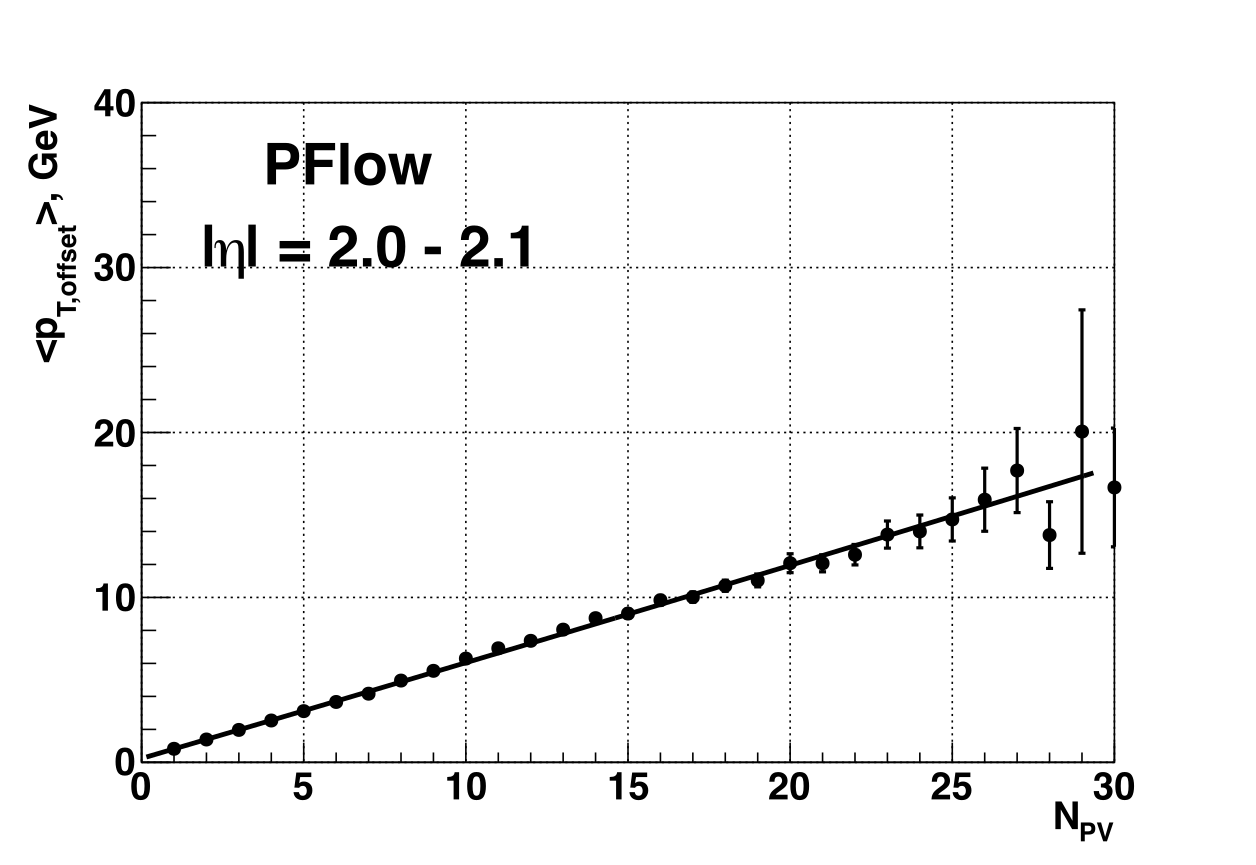
\includegraphics[width=0.45\textwidth]{chapitre4/figs/l1_offset.pdf}} \hfill
  \subcaptionbox{\label{fig:l1_offset_vs_fastjet}}[0.45\textwidth]{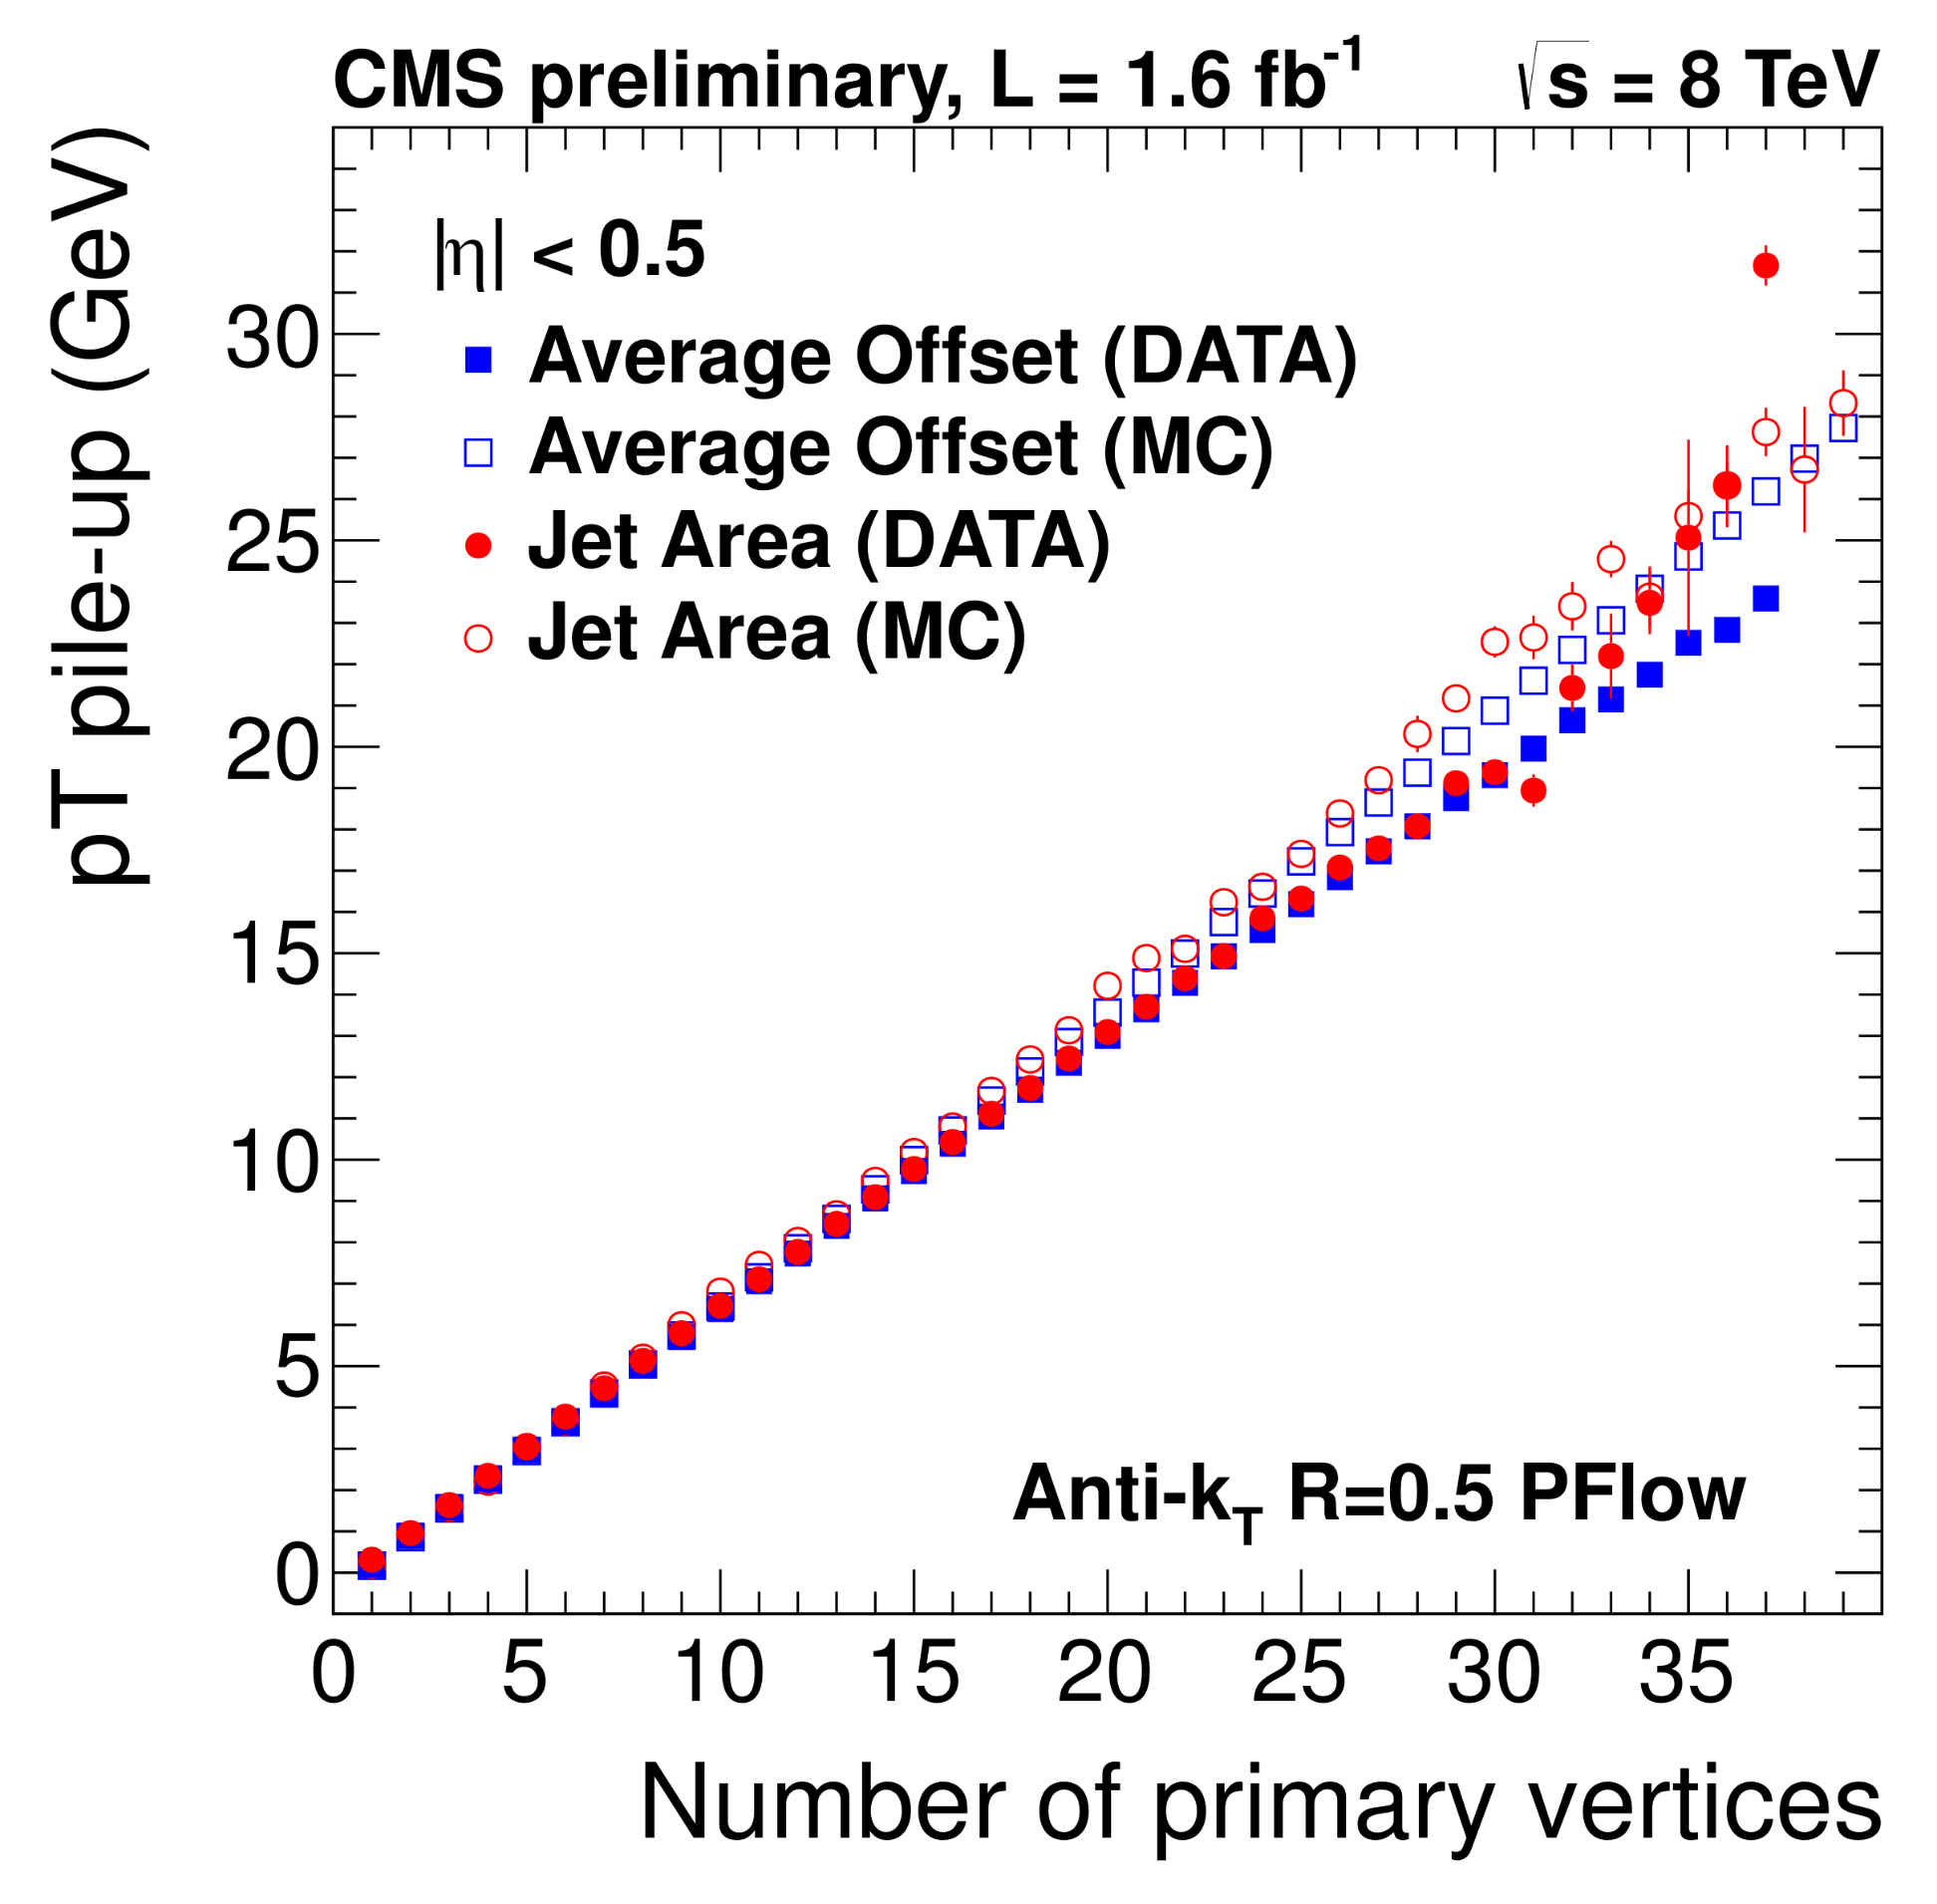
\includegraphics[width=0.45\textwidth]{chapitre4/figs/l1_offset_vs_fastjet.pdf}} \hfill
  \caption{(\subref{fig:l1_offset}) \emph{offset} en fonction du nombre de vertex primaire, pour $\num{2} < \aeta < \num{2.1}$. (\subref{fig:l1_offset_vs_fastjet}) comparaison entre les méthodes \emph{offset} et \emph{fastjet}.}
  \label{fig:jec_l1}
\end{figure}

\subsubsection{La méthode \emph{offset}}

Des événements de biais minimum sont utilisés afin d'estimer l'énergie moyenne portée par un jet à cause du \pu. Cette énergie moyenne est déterminée en fonction du nombre de vertex primaire ($N_{PV}$), une variable directement corrélée au \pu, ainsi qu'en fonction de $\aeta$ (voir \cref{fig:l1_offset}). On obtient ainsi une correction dépendante du nombre de vertex primaires, ainsi que de \aeta. Cette correction est à soustraire de l'énergie du jet afin de supprimer la contribution du \pu.

\subsubsection{La méthode \emph{fastjet}}

Il s'avère que tous les jets ne portent la même énergie due au \pu. La méthode \emph{fastjet} améliore donc la méthode \emph{offset} en ajoutant une dépendance des corrections en fonction de l'aire des jets ($A$) ainsi qu'en fonction de la densité d'énergie ($\rho$), définie comme la médiane de la distribution $p_T^j / A_j$, où $j$ est l'index d'un jet dans l'événement. La correction obtenue est donc dépendante de $\rho$, de $A$ et de \aeta. On présente \cref{fig:l1_offset_vs_fastjet} une comparaison entre ces deux méthodes.

\begin{figure}
  \subcaptionbox{\label{fig:l1_no_corr}}[0.45\textwidth]{\includegraphics[width=0.45\textwidth]{chapitre4/figs/l1_effect_no_corr.pdf}} \hfill
  \subcaptionbox{\label{fig:l1_with_corr}}[0.45\textwidth]{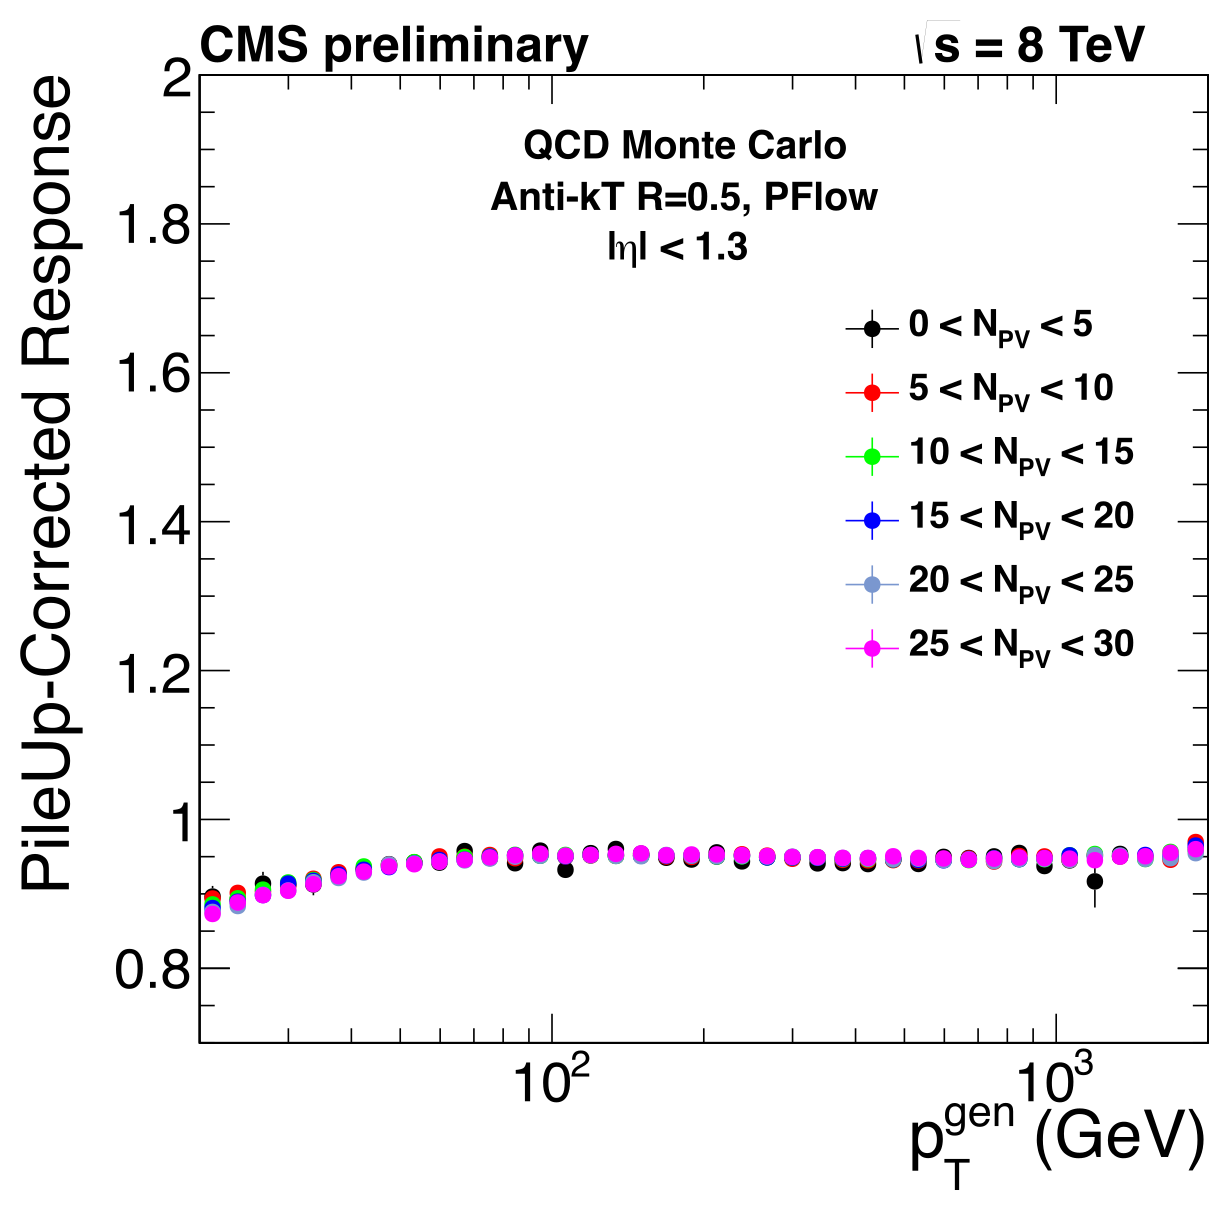
\includegraphics[width=0.45\textwidth]{chapitre4/figs/l1_effect_with_corr.pdf}} \hfill
  \caption{Évolution de la réponse des jets en fonction de l'impulsion transverse simulée, avant l'application des corrections de niveau 1 (\subref{fig:l1_no_corr}) et après (\subref{fig:l1_with_corr}), pour différentes classes de $N_{PV}$.}
  \label{fig:jec_l1_effect}
\end{figure}

\bigskip

Après application des corrections de niveau 1, la réponse des jets, définie comme le rapport en l'impulsion transverse du jet sur l'impulsion transverse vraie, n'est plus dépendante du nombre de vertex primaires, comme on peux le voir \cref{fig:l1_with_corr}.

\subsection{Les corrections de niveau 2 et 3}

Ces corrections sont appliquées après celles de niveau 1. La réponse n'est donc plus dépendante du \pu. Néanmoins, elle varie toujours en fonction de \aeta et du $p_T$. Afin de corriger ces effets, on utilise des événements di-jets, contenant seulement 2 jets. Par conservation de l'impulsion transverse, on a donc $p_T^\text{jet 1} = p_T^\text{jet 2}$. De plus, on considère que les jets dans la région centrale du détecteur ($\aeta < \num{1.3}$) sont correctement reconstruit. On sélection donc des événements avec au moins un jet dans la région centrale, et on calcule la réponse $R$, définie comme $p_T^\text{jet} / p_T^\text{central}$, en fonction de \aeta et $p_T$. Dans le cas d'une reconstruction parfaite, la réponse vaut 1. Dans le cas contraire, le facteur de correction à appliquer est $1 / R$.

%\begin{figure}
  %\subcaptionbox{\label{fig:l2l3_response}}[0.45\textwidth]{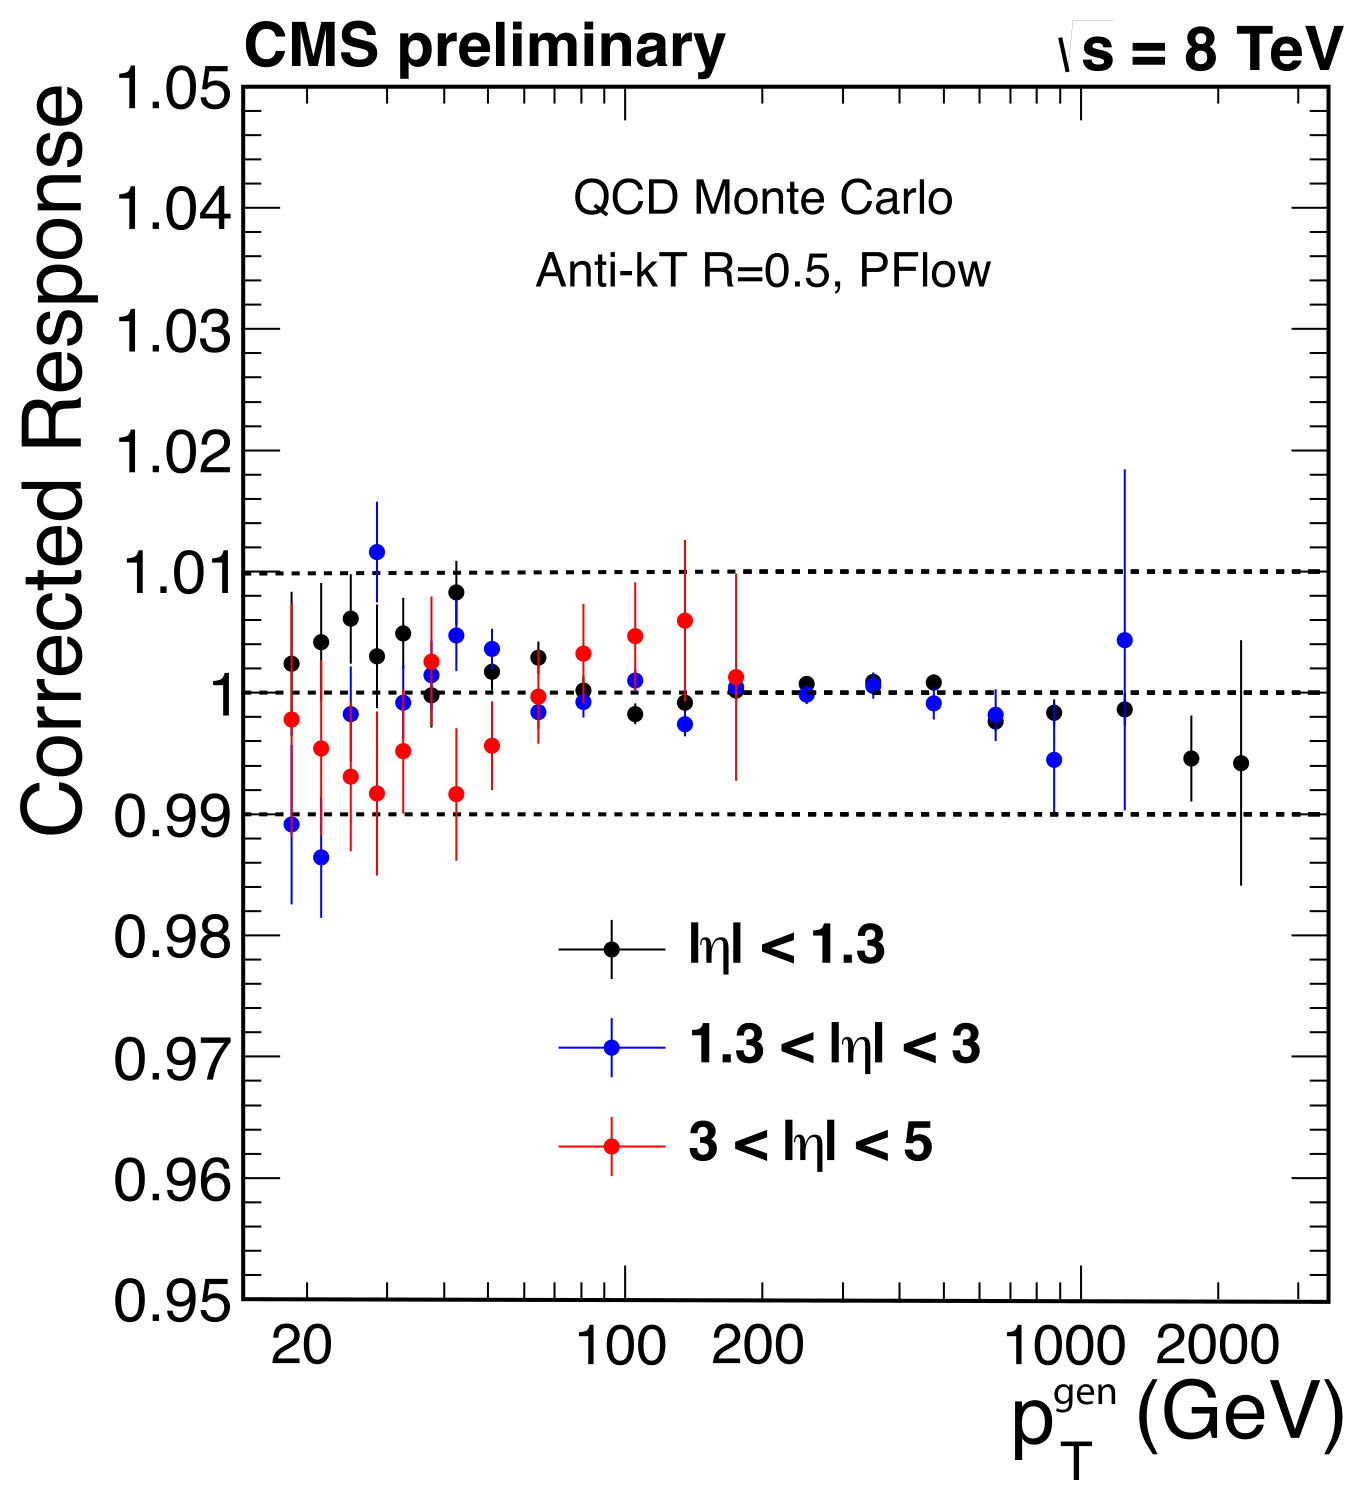
\includegraphics[width=0.45\textwidth]{chapitre4/figs/l2l3_response.pdf}} \hfill
  %\subcaptionbox{\label{fig:l1l2l3}}[0.45\textwidth]{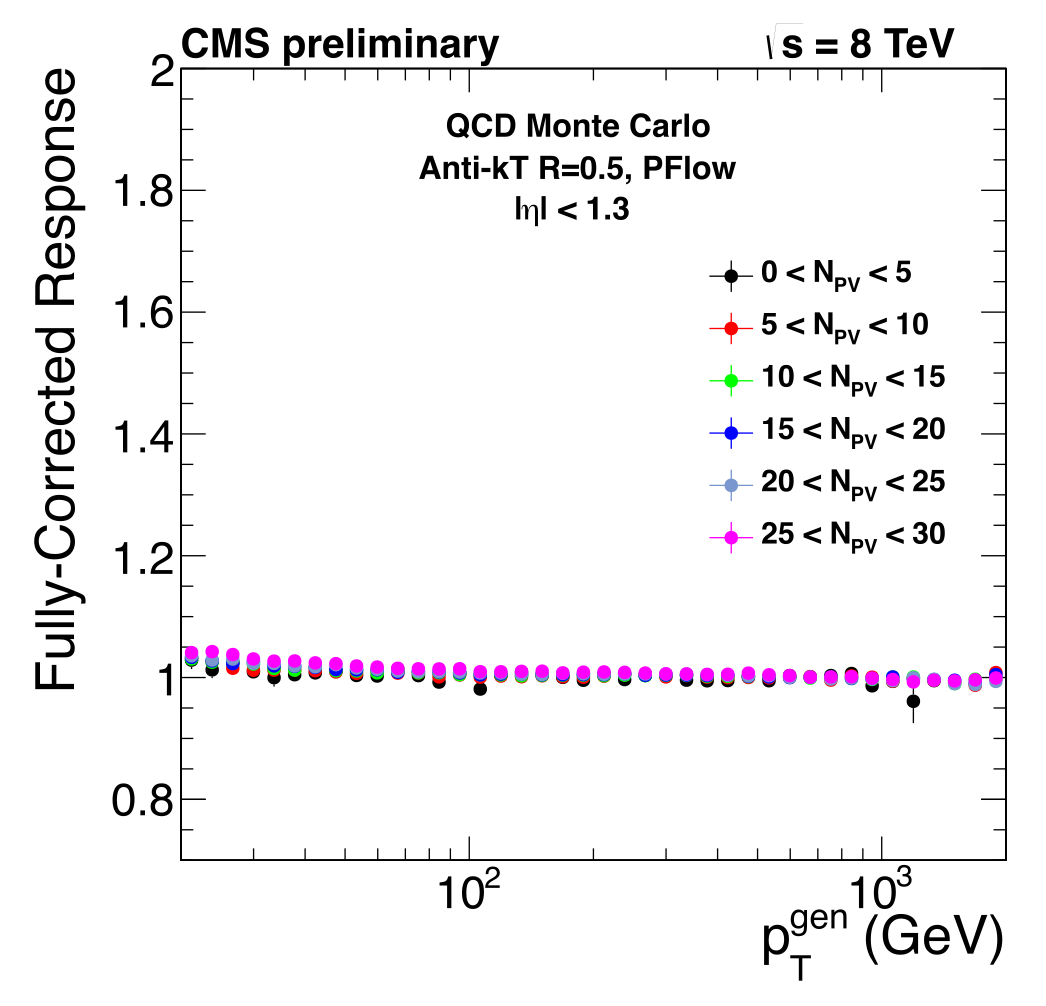
\includegraphics[width=0.45\textwidth]{chapitre4/figs/response_after_l1l2l3.pdf}} \hfill
  %\caption{Évolution de la réponse des jets en fonction de l'impulsion transverse simulée, avant l'application des corrections de niveau 1 (\subref%{fig:l1_no_corr}) et après (\subref{fig:l1_with_corr}), pour différentes classes de $N_{PV}$.}
%  \label{fig:jec_l2l3}
%\end{figure}

\begin{figure}[tbp]
    \centering
    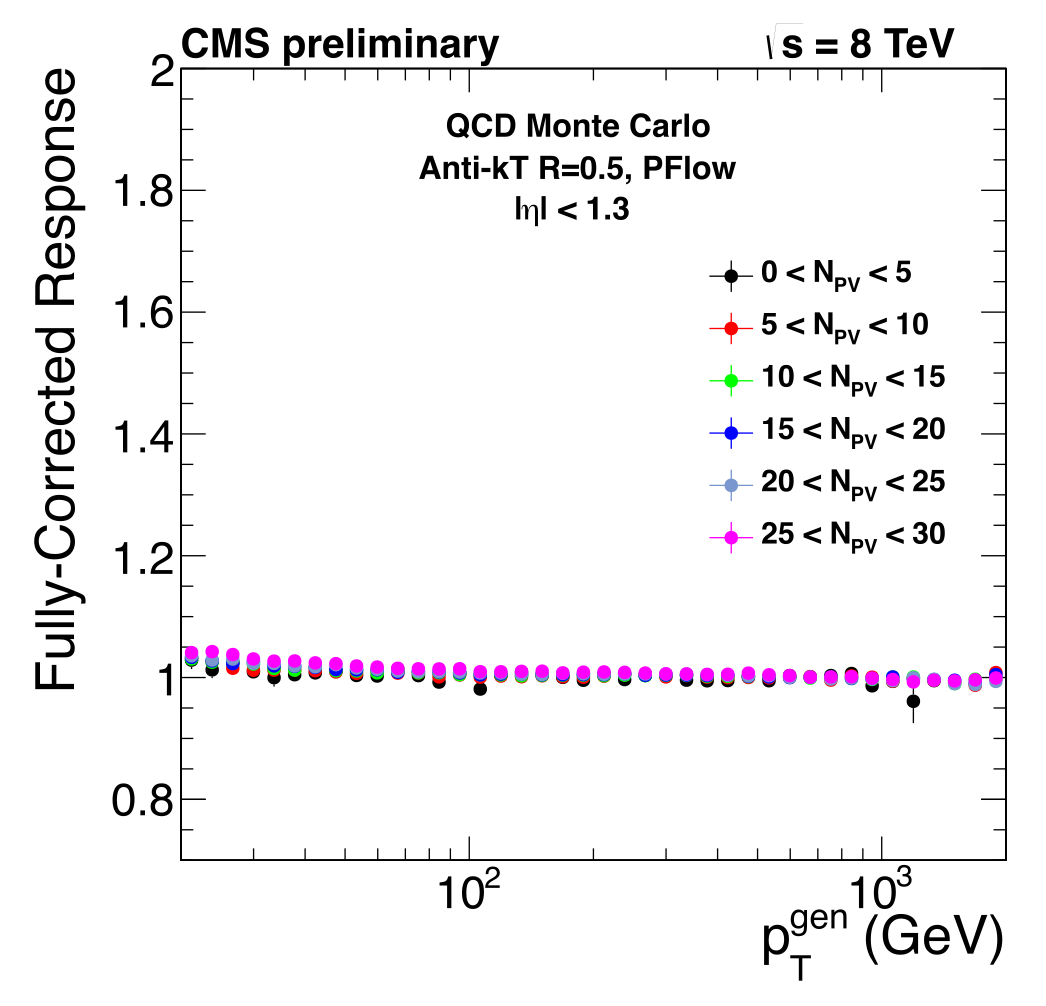
\includegraphics[width=0.55\textwidth]{chapitre4/figs/response_after_l1l2l3.pdf}
    \caption{Réponse des jets après application des corrections de niveau 1, 2 et 3, pour des événements QCD simulés}
    \label{fig:resp_l1l2l3}
\end{figure}

On présente \cref{fig:resp_l1l2l3} la réponse des jets après application des corrections de niveau 1, 2 et 3, pour des événements QCD simulés. La réponse est maintenant linéaire.

\subsection{Les corrections résiduelles}

Les corrections précédentes sont toutes dérivées à l'aide de la simulation. Malheureusement, cette simulation n'est pas parfaite, et des différences existent entre la réponse des jets dans la simulation et dans les données collectées. On applique ainsi un autre niveau de corrections, uniquement sur les données, afin de corriger des dernières différences entre données et simulation. Ces corrections, dépendante de \aeta et du $p_T$ des jets, sont déterminées à l'aide d'événement $\PZ \rightarrow \left[ \Pmuon \APmuon \, | \, \Pelectron \APelectron \right] $ + jets ou $\Pphoton$ + jets.

Ayant fait l'objet de ma tâche de service au sein de CMS, la détermination des corrections résiduelles à l'aide d'événement $\Pphoton$ + jets est décrite en détails dans la section suivante.

\section{Détermination des corrections résiduelles à l'aide d'événements \texorpdfstring{$\Pphoton$}{γ} + jets}

\subsection{Intérêt des événements \texorpdfstring{$\Pphoton$}{γ} + jets}

On cherche à corriger des dernières différences entre simulation et données collectées. Pour cela, on mesure la réponse des jets dans les données, ainsi que dans la simulation, et on corrige les données pour coller à la simulation. Il est donc nécessaire d'utiliser un processus physique qui permet de connaître de façon certain l'énergie d'un jet, sans avoir pour cela à utiliser la vérité de la simulation.

\begin{figure}[t!] \centering
  \subcaptionbox{\label{fig:g_plus_jet_1}}[.4\linewidth]{
  \begin{fmfgraph*}(180,120)
    \fmfpen{0.5}
    \fmfleft{i1,i2}
    \fmfright{o1,o2}
    \fmf{gluon}{i1,v1}
    \fmf{fermion}{i2,v1}
    \fmf{fermion,label=\Pquark}{v1,v2}
    \fmf{fermion}{v2,o1}
    \fmf{photon}{v2,o2}
    \fmffreeze
    \fmfdot{v1,v2}
    \fmflabel{\Pquark}{i2}
    \fmflabel{\Pquark}{o1}
    \fmflabel{\Pphoton}{o2}
  \end{fmfgraph*}}\qquad \quad%
  % \begin{fmfgraph*}(180,120)
  %   \fmfpen{0.5}
  %   \fmfleft{i1,i2}
  %   \fmfright{o1,o2,o3}
  %   \fmf{gluon}{i2,v1}
  %   \fmf{gluon}{v3,o1}
  %   \fmf{fermion}{i1,v3}
  %   \fmf{fermion,label=\APquark}{v3,v2,v1}
  %   \fmf{fermion}{v1,o3}
  %   \fmffreeze
  %   \fmf{photon,label=\Pphoton}{v2,o2}
  %   \fmfdot{v1,v2,v3}
  %   \fmflabel{\Pquark}{i1}
  %   \fmflabel{\Pquark}{o3}
  % \end{fmfgraph*}}\qquad \quad%
  \subcaptionbox{\label{fig:g_plus_jet_2}}[.4\linewidth]{
  \begin{fmfgraph*}(180,120)
    \fmfpen{0.5}
    \fmfstraight
    \fmfleft{i1,i2}
    \fmfright{o1,o2,o3}
    \fmf{fermion}{i1,v1,i2}
    \fmf{fermion}{v4,v2}
    \fmf{phantom}{o1,v4}
    \fmf{fermion,label=\Pquark}{v2,v3}
    \fmf{photon,label=$\Pphoton$}{v3,o3}
    \fmf{gluon}{v1,v2}
    \fmffreeze
    \fmf{fermion}{v3,o2}
    \fmfdot{v1,v2,v3}
    \fmflabel{\APquark}{i2}
    \fmflabel{\Pquark}{i1}
    \fmflabel{\Pquark}{o2}
    \fmflabel{\APquark}{v4}
  \end{fmfgraph*}
  }
  \caption{Diagrammes de Feynman associés à la production d'un photon et d'un jet (\subref{fig:g_plus_jet_1}) et d'un photon et de deux jets (\subref{fig:g_plus_jet_2}).}
  \label{fig:gamma_jet_diagrams}
\end{figure}

On utilise des processus comportant uniquement deux particules dans l'état final : une particule dont on connaît très bien les propriétés (boson \PZ, photon, \ldots), qui sera notre sonde, et un jet. On utilise ensuite les propriétés de la sonde pour déterminer celles du jet. Dorénavant, on se concentrera uniquement sur les événements \Pphoton + jets.

\bigskip

On présente \cref{fig:gamma_jet_diagrams} deux diagrammes de Feynman représentant la production d'un photon accompagné d'un ou deux jets. L'impulsion dans le plan transverse étant nulle au moment de la collision, on a, dans l'état final
\begin{align*}
  \vec{p}_T &= 0 = \vec{p}_{T}^{\Pphoton} + \vec{p}_T^\text{jet}\\
  \norm{\vec{p}_T^{\Pphoton}} &= \norm{\vec{p}_T^{jet}}
\end{align*}

Ainsi, il est suffisant de connaître l'impulsion transverse de la sonde pour déterminer l'impulsion transverse du jet. Le calorimètre électromagnétique étant bien plus performant que le calorimètre hadronique, on voit ici tout l'intérêt du choix du photon comme sonde.

\subsection{Détermination de la réponse des jets}

On cherche à déterminer la réponse $R$ des jets
%c'est-à-dire le rapport $R = p_T^\text{jet} / p_T^{\Pphoton}$
, qui tend vers 1 si l'on reconstruit parfaitement le jet. On utilise deux méthodes différentes pour déterminer cette réponse : la méthode de la balance, et la méthode MPF, détaillée ci-dessous.

\subsubsection{La méthode de la balance}

On utilise le principe de conservation de l'impulsion transverse. On a alors
\begin{align*}
  \norm{\vec{p}_T^{\Pphoton}} &= \norm{\vec{p}_T^{jet}}
\end{align*}
et on défini la réponse $R$ par la relation
\begin{align*}
    R &= \frac{p_T^\text{jet}}{p_T^{\Pphoton}}
\end{align*}

Cette méthode est très simple et performante. Néanmoins, elle est très sensible au \pu, ainsi qu'aux radiations dans l'état final. En effet, la présence d'autres jets dans l'état final vont venir perturber la balance entre le jet et le photon. On verra par la suite comment restaurer cette balance.

\subsubsection{La méthode MPF (\emph{Missing $E_T$ projection fraction})}

Un événement \Pphoton + jets n'a pas de \met. Ainsi, au niveau partonique, on a
\begin{align*}
  \vec{p}_T^{\Pphoton} + \vec{p}_T^{\text{recul}} &= -\vec{\met} = \vec{0}
\end{align*}
où $\vec{p}_T^{\text{recul}}$ est le vecteur impulsion transverse de tous les autres particules dans l'événement.

Après reconstruction, on a
\begin{align*}
  R_{\Pphoton} \, \vec{p}_T^{\Pphoton} + R_{\text{recul}} \, \vec{p}_T^{\text{recul}} &= -\vec{\met}
\end{align*}
$R_X$ désigne ici la réponse des détecteurs lors de la reconstruction de l'objet $X$.

On considère que les photons sont reconstruits de façon parfaite, on pose donc $R_{\Pphoton} = 1$. En utilisant le fait que $\vec{p}_T^{\text{recul}} = -\vec{p}_T^{\Pphoton}$ on obtient
\begin{align*}
  R_{\text{recul}} &= 1 + \frac{\vec{\met} \cdot \vec{p}_T^{\Pphoton}}{\left( p_T^{\Pphoton} \right)^2} \equiv R_{\text{MPF}}
\end{align*}

Cette méthode n'est pas dépendante de la présence de jets additionnels dans l'événement, mais requiert par contre une excellente reconstruction de l'énergie transverse manquante. C'est le cas dans CMS grâce à l'utilisation de l'algorithme du \pf.

\medskip

Cette méthode est utilisée pour produire les corrections officielles. La méthode de la balance permet de vérifier la compatibilité des corrections obtenues.

\subsubsection{L'extrapolation}

La balance entre le photon et le jet est perturbée par la présence de jets additionnels dans l'événement, provenant soit du \pu, soit de radiations dans l'état final. On définit $\alpha$ comme le rapport entre l'impulsion transverse du second jet de l'événement sur l'impulsion transverse du photon,
\begin{align}
    \alpha &= \frac{p_T^{\text{\ordinalnum{2} jet}}}{p_T^\gamma}
\end{align}

Afin de réduire la dépendance de la réponse à la présence de jets additionnels, on effectue un découpage de la réponse en $\alpha$, et on extrapole le comportement de la réponse pour $\alpha \rightarrow 0$. On verra plus loin que cette extrapolation est très efficace pour la réponse obtenue avec la méthode de la balance, et inutile pour la méthode MPF.

\end{fmffile}

\subsection{Sélection des événements}

\begin{figure}[tbp]
    \centering
    \includegraphics[width=0.5\textwidth]{chapitre4/figs/pu_plot.pdf}
    \caption{Distribution du nombre moyen d'interactions par croisement de faisceaux pour deux chemins de déclenchement, \emph{HLT\_Photon30\_CaloIdVL\_IsoL} (rouge) et \emph{HLT\_Photon150} (bleu)}
    \label{fig:label}
\end{figure}

On cherche à sélectionner des événements contenant un unique photon, ainsi qu'un ou deux jets. Le principal bruit de fond est dû aux événements multi-jets (de type $\Pquark \APquark \rightarrow \Pquark \APquark$) où un jet est identifié incorrectement comme un photon. On utilise comme signal des événements $\Pphoton$ + jets simulés.

Afin d'éliminer une grande partie du bruit du fond, une sélection est appliquée. La première étape consiste à sélectionner des événements contenant uniquement un seul photon. On utilise pour cela une méthode d'identification des photons fournie par la collaboration. Cette méthode est disponible selon trois points de fonctionnement, selon si l'on est intéressé par une grande efficacité ou par une grande pureté. Le point de fonctionnement choisi est le point qui offre la plus grande pureté ($\tilde \SI{96}{\%}$), au détriment de l'efficacité ($\tilde \SI{70}{\%}$). Cette identification est définie de la façon suivante :

\begin{enumerate}
    \item Un contrôle est effectué pour vérifier que le photon n'est pas en réalité un électron, et qu'il ne provient pas de la conversion d'un électron lors de son passage dans le ECAL.
    \item Le ratio de l'énergie collectée dans le calorimètre hadronique sur l'énergie collectée dans le calorimètre électromagnétique doit être inférieur à \SI{5}{\%}. La majorité de l'énergie doit donc être déposée dans le calorimètre électromagnétique.
    \item $\sigma_{i\eta i\eta} < \num{0.011}$. Cette variable est caractéristique de la forme de la gerbe électronique dans le calorimètre électromagnétique, plus étalée dans le cas d'un électron que d'un photon. \fxnote{Définition ? Voir \url{https://indico.cern.ch/event/27560/material/slides/1?contribId=1}}
\end{enumerate}

En plus de ces trois critères, on demande à ce que le photon soit isolé. On défini l'isolation $I$ comme le rapport entre l'énergie de toutes les particules \pf contenue dans un cône de rayon $\Delta R = \num{0.3}$ centré autour du photon, divisé par l'énergie du photon. Cette valeur est hautement sensible au \pu. On applique ainsi une procédure qui permet de diminuer l'impact du \pu, en corrigeant cette isolation par un facteur dépendant de la densité d'énergie $\rho$. On a ainsi $I_\text{corr} = \max{\left(I - f(\rho), 0\right)}$. On effectue des coupures sur cette isolation selon trois différents type de particules : les hadrons neutres, chargés, et les photons :

\begin{itemize}
    \item $I_\text{hadrons neutres} < \num{0.4} + \num{0.04} \, p_T^{\Pphoton}$
    \item $I_\text{hadrons chargés} < \num{0.7}$
    \item $I_\text{photons} < \num{0.5} + \num{0.005} \, p_T^{\Pphoton}$
\end{itemize}

Afin de ne garder que les photons les mieux reconstruits, on sélectionne uniquement ceux reconstruit dans le tonneau, avec $\aeta < \num{1.3}$, et une impulsion transverse d'au moins \SI{40}{\GeV}.

\medskip

On demande en plus au moins un bon jet dans l'événement. Cette identification est très efficace ($> \SI{99}{\%}$) et permet d'éliminer les faux jets dû à des bruits dans les détecteurs. La séparation azimutale $\abs{\Delta \phi}$ dans le plan transverse entre le photon et le premier jet de l'événement doit être supérieure à \SI{2.8}{\radian}, afin de ne conserver que les événements où le photon et le jet sont dos-à-dos. On présente \cref{fig:schema_gamma_jet,fig:schema_gamma_jets} une représentation graphique d'un événement $\Pphoton$ + jets avec 1 ou 2 jets. Dans le cas où un second jet est présent, on vérifie que son énergie est inférieure à \SI{20}{\%} de celle du photon ($\alpha < \num{0.20}$), afin d'éviter de conserver des événements trop déséquilibré. Cette condition n'est appliquée que si $p_T^{\text{\ordinalnum{2} jet}} \geq \SI{10}{\GeV}$. Tous les jets sont corrigés avec les corrections de niveau 1, 2 et 3. Cependant, les corrections résiduelles ne sont pas appliquées sur les données puisque ce sont ces corrections que l'on souhaite déterminer au travers de cette analyse.

\begin{figure}[tbp] \centering
  \subcaptionbox{\label{fig:schema_gamma_jet}}[0.45\textwidth]{\scalebox{2}{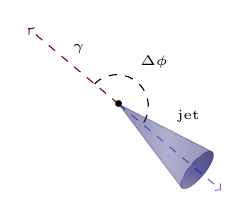
\begin{tikzpicture}[rotate=45]
    \draw[draw=red!50!black,dashed,->] (0:0) -- (95:1.5) ;
    \draw (90:1) node[right] {\tiny $\gamma$} ;

    \draw[draw=blue!60,dashed,->] (0:0) -- (-85:1.7) ;

    \draw[dashed] (95:4mm) arc (90:-80:4mm) ;
    \draw (5:7mm) node {\tiny $\Delta\phi$} ;

    \begin{scope}[rotate=5]
      \fill[top color=blue!50!black,bottom color=blue!10,middle color=blue,shading=axis,opacity=0.25] (0,-13mm) circle (3mm and 1mm);
      \fill[left color=blue!50!black,right color=blue!50!black,middle color=blue!50,shading=axis,opacity=0.25] (3mm,-13mm) -- (0,0mm) -- (-3mm,-13mm) arc (180:360:3mm and 1mm);
      \draw[draw=blue!50!black,opacity=0.25] (-3mm,-13mm) arc (180:360:3mm and 1mm) -- (0,0mm) -- cycle;
      \draw[draw=blue!50!black,opacity=0.25,densely dashed] (-3mm,-13mm) arc (180:0:3mm and 1mm);
    \end{scope}

    \draw (-55:0.9) node {\tiny jet} ;
    \draw (0:0) node {\tiny $\bullet$} ;

  \end{tikzpicture}}} \quad
  \subcaptionbox{\label{fig:schema_gamma_jets}}[0.45\textwidth]{\scalebox{2}{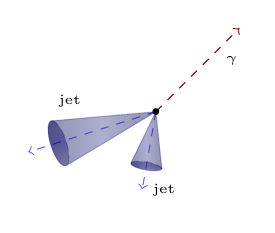
\begin{tikzpicture}
    \draw[draw=red!50!black,dashed,->] (0:0) -- (45:1.5) ;
    \draw (40:1) node[right] {\tiny $\gamma$} ;

    \draw[draw=blue!60,dashed,->] (0:0) -- (-100:1) ;
    \draw[draw=blue!60,dashed,->] (0:0) -- (-162.5:1.7) ;

    \begin{scope}[rotate=-72]
      \fill[top color=blue!50!black,bottom color=blue!10,middle color=blue,shading=axis,opacity=0.25] (0,-13mm) circle (3mm and 1mm);
      \fill[left color=blue!50!black,right color=blue!50!black,middle color=blue!50,shading=axis,opacity=0.25] (3mm,-13mm) -- (0,0mm) -- (-3mm,-13mm) arc (180:360:3mm and 1mm);
      \draw[draw=blue!50!black,opacity=0.25] (-3mm,-13mm) arc (180:360:3mm and 1mm) -- (0,0mm) -- cycle;
      \draw[draw=blue!50!black,opacity=0.25,densely dashed] (-3mm,-13mm) arc (180:0:3mm and 1mm);
    \end{scope}

    \begin{scope}[rotate=-10]
      \fill[top color=blue!50!black,bottom color=blue!10,middle color=blue,shading=axis,opacity=0.25] (0,-7mm) circle (2mm and 0.5mm);
      \fill[left color=blue!50!black,right color=blue!50!black,middle color=blue!50,shading=axis,opacity=0.25] (2mm,-7mm) -- (0,0mm) -- (-2mm,-7mm) arc (180:360:2mm and 0.5mm);
      \draw[draw=blue!50!black,opacity=0.25] (-2mm,-7mm) arc (180:360:2mm and 0.5mm) -- (0,0mm) -- cycle;
      \draw[draw=blue!50!black,opacity=0.25,densely dashed] (-2mm,-7mm) arc (180:0:2mm and 0.5mm);
    \end{scope}

    \draw (-84:1) node {\tiny jet} ;
    \draw (-187:1.1) node {\tiny jet} ;
    \draw (0:0) node {\tiny $\bullet$} ;

  \end{tikzpicture}}}
  \caption{Un événement $\gamma$ + jets parfaitement dos-à-dos (\subref{fig:schema_gamma_jet}) et où la balance est brisée (\subref{fig:schema_gamma_jets}).}
  \label{fig:schema_g_jet}
\end{figure}

Pour terminer la sélection, un véto est imposé sur la présence d'électrons ou de muons dans l'événement. Sur des événements de signal simulés, cette sélection a une efficacité de \SI{20.26}{\%}, et de \SI{0.02}{\%} sur le bruit de fond. On présente \cref{fig:pt_photon_jet} une comparaison entre la simulation et les données pour l'impulsion transverse du photon, du premier jet de l'événement, du second, ainsi que l'énergie transverse manquante.

\begin{figure}[p]
    \centering
    \subcaptionbox{\label{pt_photon}}[0.45\textwidth]{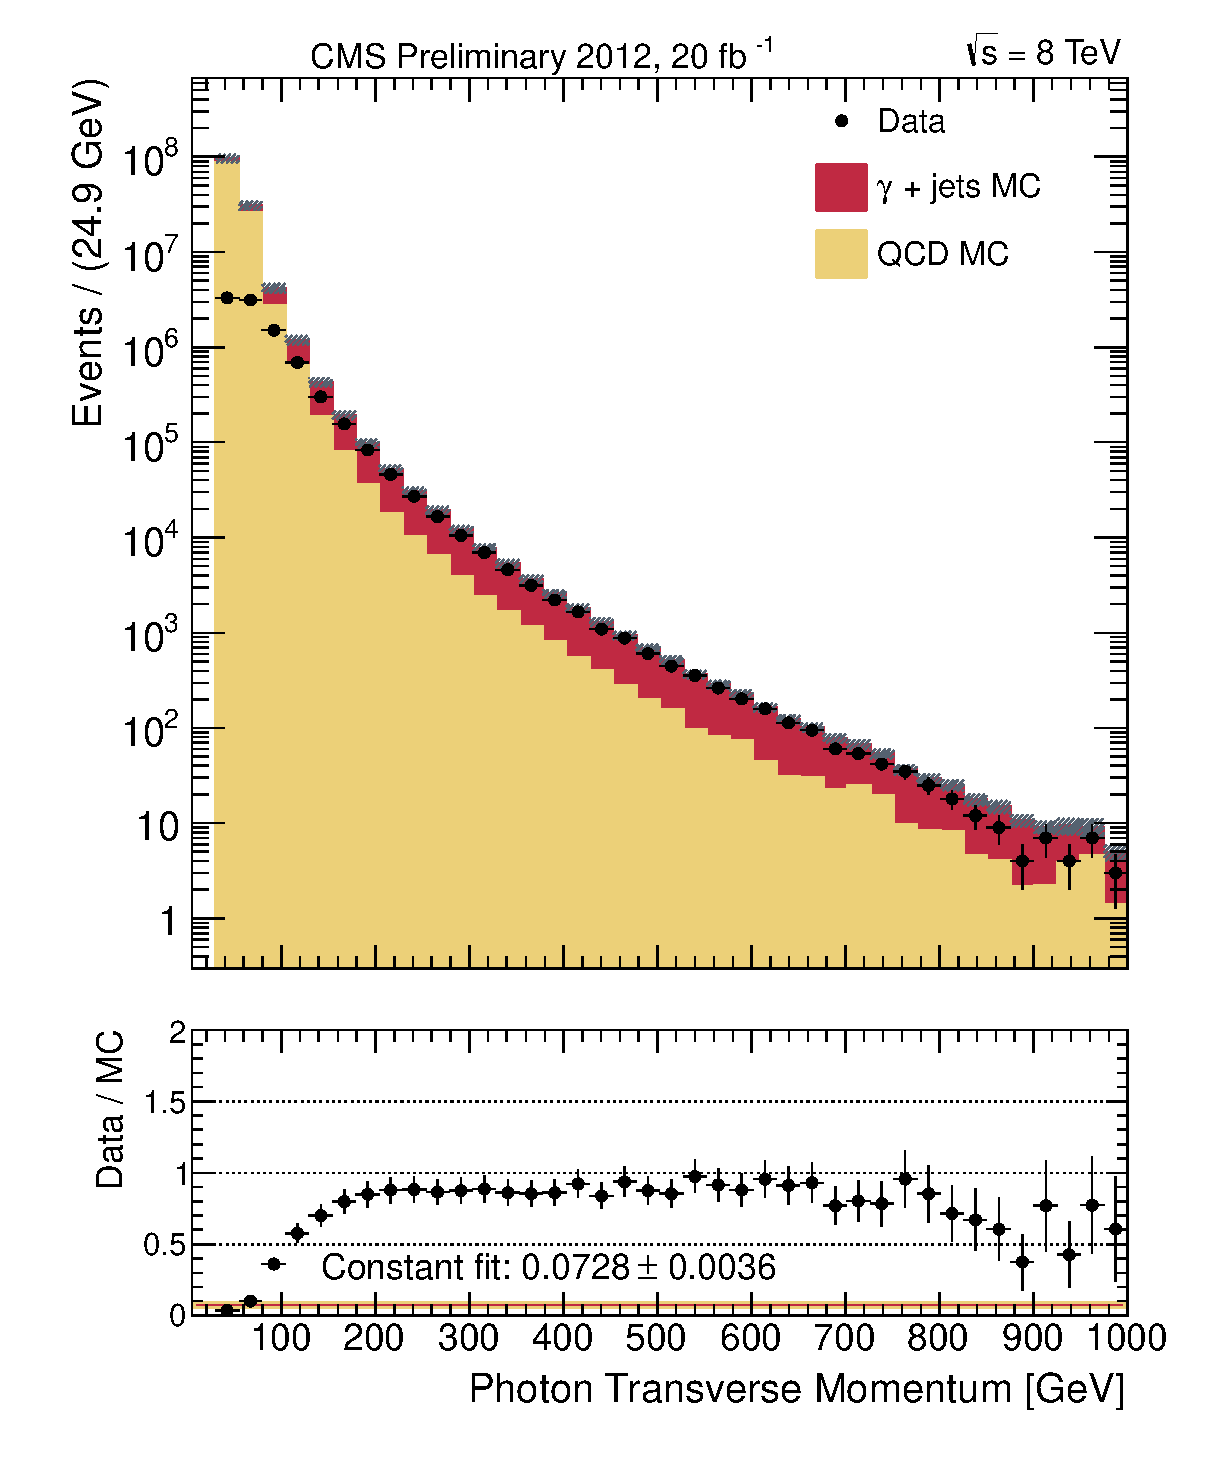
\includegraphics[width=0.45\textwidth]{chapitre4/figs/ptPhoton_passedID_log.eps}}\hfill
    \subcaptionbox{\label{pt_first_jet}}[0.45\textwidth]{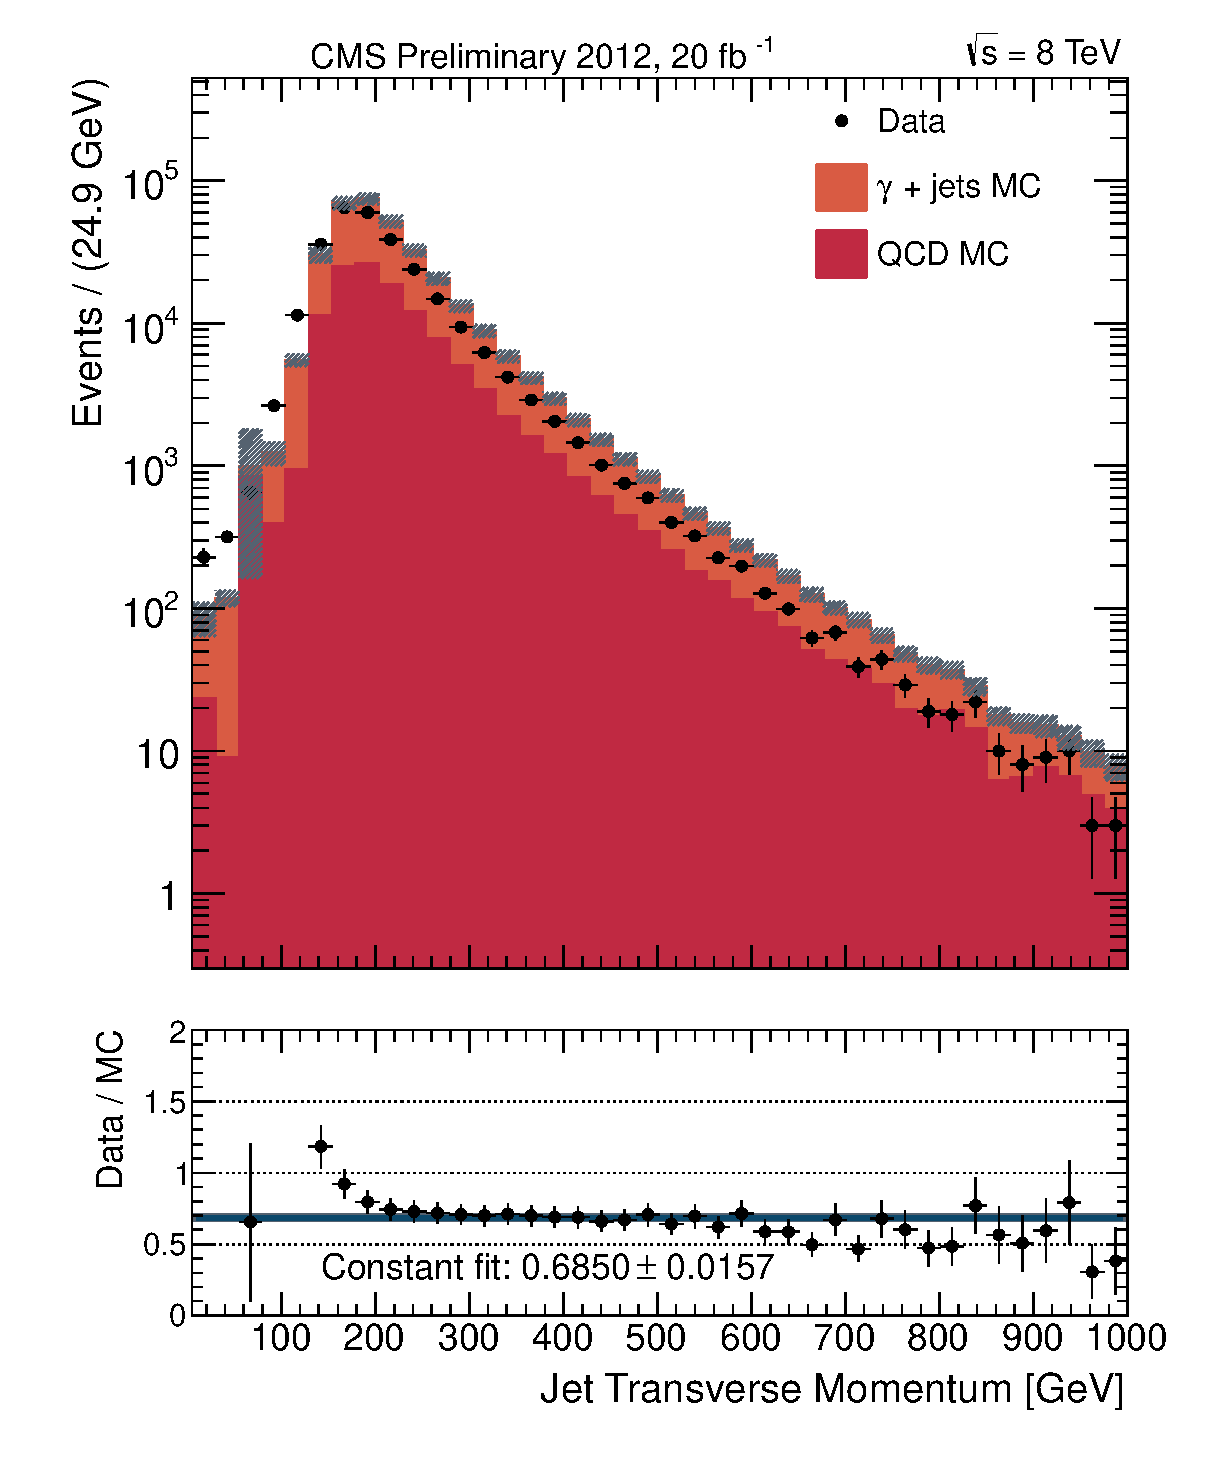
\includegraphics[width=0.45\textwidth]{chapitre4/figs/ptFirstJet_passedID_log.eps}}
    \subcaptionbox{\label{pt_second_jet}}[0.45\textwidth]{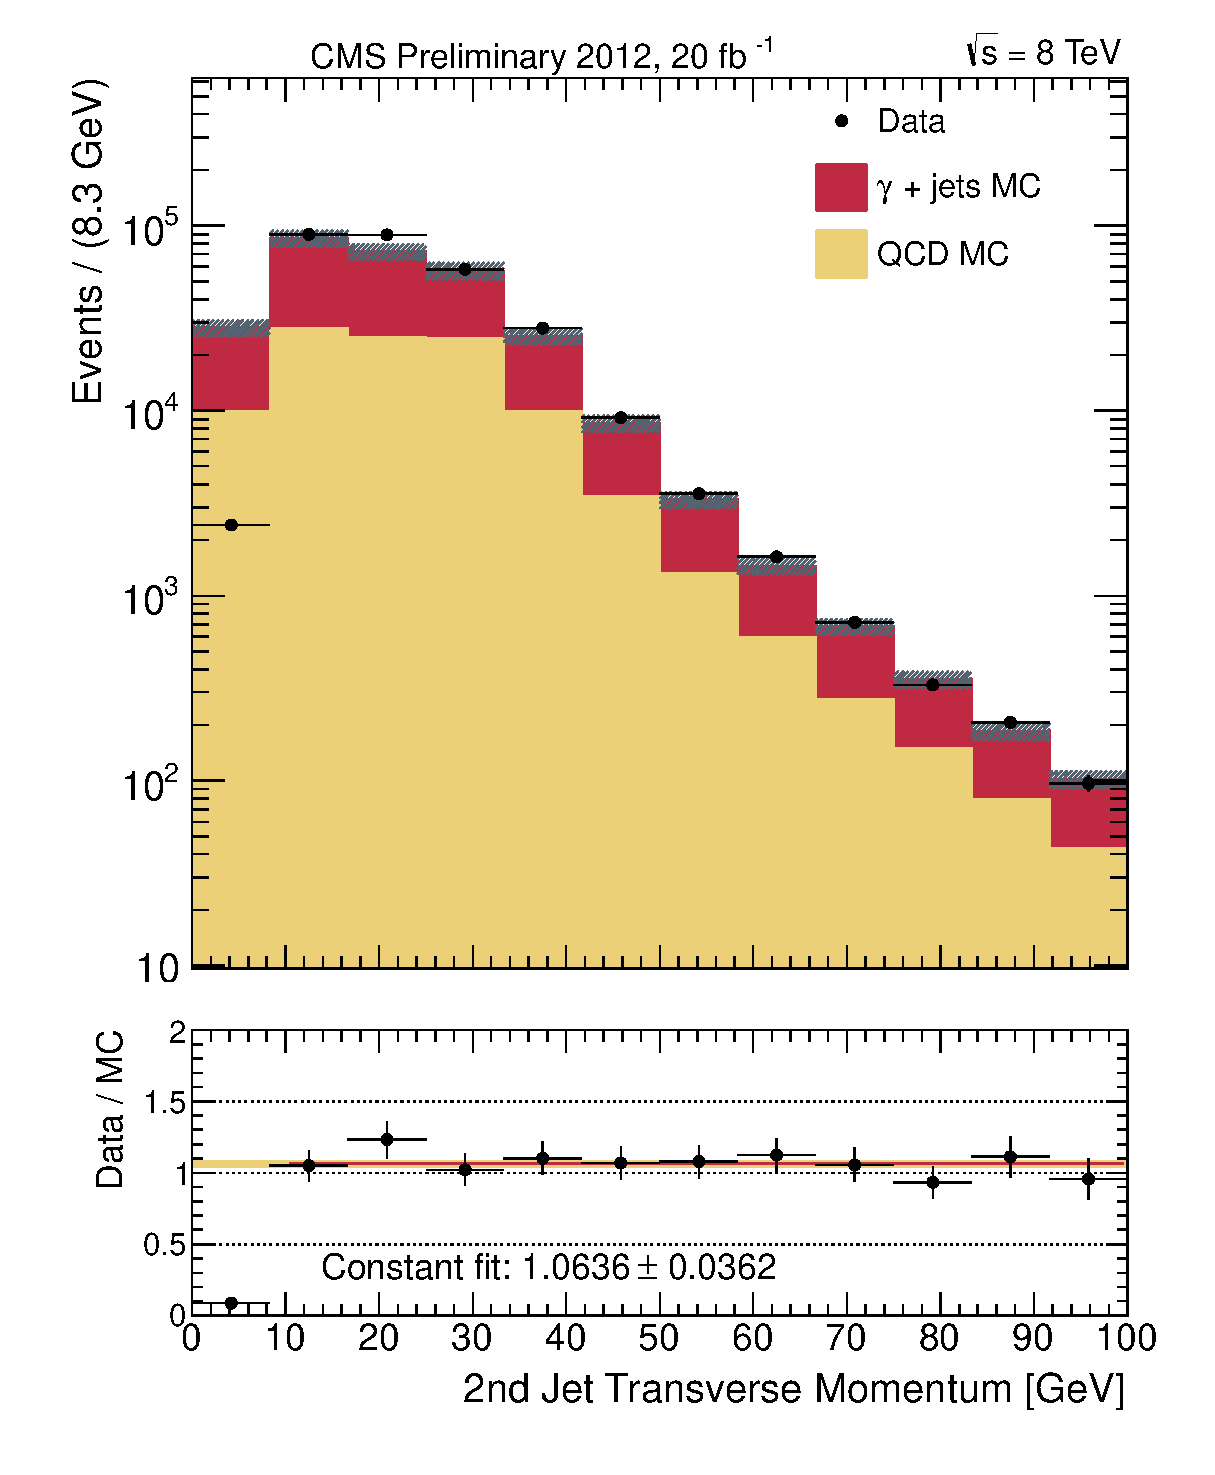
\includegraphics[width=0.45\textwidth]{chapitre4/figs/ptSecondJet_passedID_log.eps}}\hfill
    \subcaptionbox{\label{met}}[0.45\textwidth]{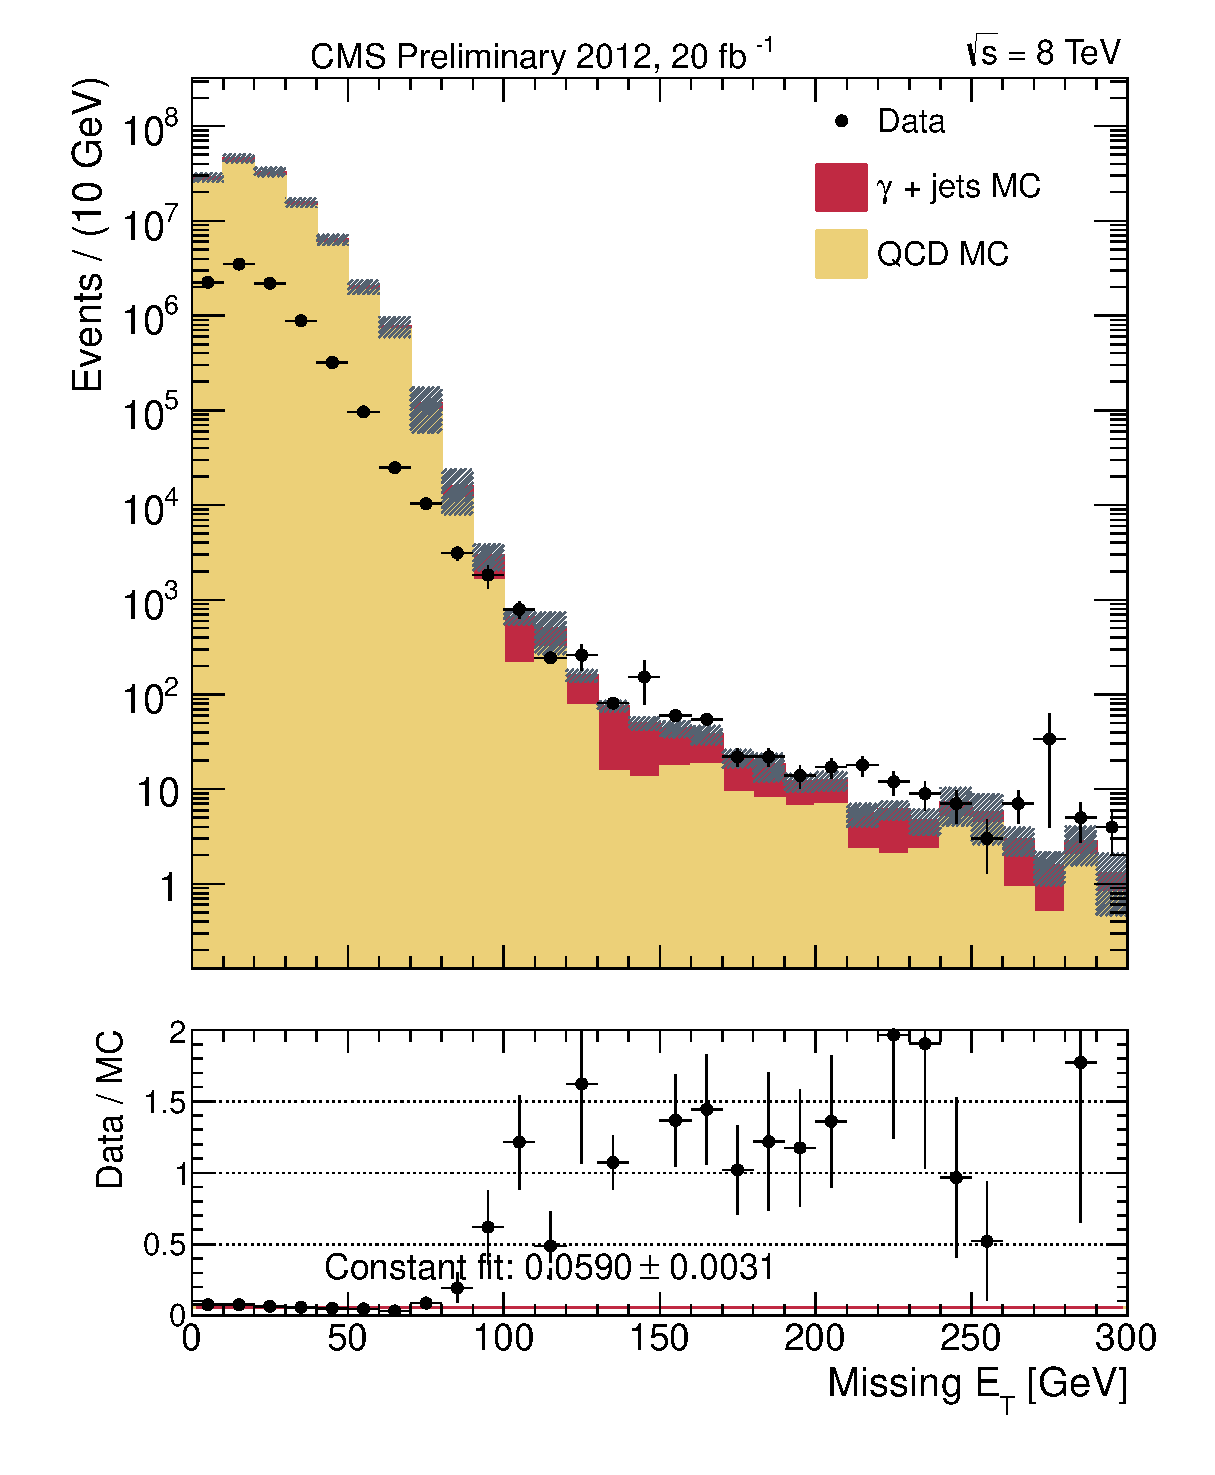
\includegraphics[width=0.45\textwidth]{chapitre4/figs/MET_passedID_log.eps}}
    \caption{Comparaison entre la simulation (histogrammes) et les données (points) pour l'impulsion transverse du photon (\subref{pt_photon}), pour le premier jet de l'événement (\subref{pt_first_jet}), le second (\subref{pt_second_jet}) ainsi que l'énergie transverse manquante (\subref{met}) après sélection. Une coupure additionnelle sur l'impulsion transverse du photon à \SI{165}{\GeV} a été appliquée pour éviter les effets des \emph{prescales} des chemins de déclenchements. \fxerror{corriger}.}
    \label{fig:pt_photon_jet}
\end{figure}

\bigskip

Sur les données, on demande à ce que les événements aient déclenchés les chemins de déclenchements demandant un bon photon isolé. Plusieurs chemins de déclenchements existent suivant l'impulsion du photon demandé, dont la plupart préscalés. Afin de pouvoir comparer les données et la simulation sans être gêné par le préscale, on applique une coupure supplémentaire sur l'impulsion transverse du photon à \SI{175}{\GeV}. Cette coupure n'est pas appliquée pour déterminer les facteurs de corrections, mais uniquement pour comparer les distributions.

\smallskip

Finalement, la simulation des événements QCD et $\gamma$ + jets a été effectuée pendant la prise de données. A cette époque, le profile de \pu n'était pas encore connu précisément. Ainsi, une estimation de ce profile a été utilisé pour la simulation. On repondère donc le profile de \pu de la simulation pour qu'il corresponde à celui observé sur les données collectées.

\subsection{Stratégie d'analyse}

On effectue un découpage suivant l'impulsion transverse du photon et de sa position angulaire, afin d'augmenter la sensibilité de l'analyse. Pour l'impulsion transverse, on définit 14 classes :

\setlength{\columnsep}{0pt}
\begin{multicols}{4}
  \begin{itemize} \setlength{\itemsep}{0.4\itemsep}
      \item 40 - \SI{50}{\GeV}
      \item 50 - \SI{60}{\GeV}
      \item 60 - \SI{75}{\GeV}
      \item 100 - \SI{125}{\GeV}
      \item 125 - \SI{155}{\GeV}
      \item 155 - \SI{180}{\GeV}
      \item 180 - \SI{210}{\GeV}
      \item 250 - \SI{300}{\GeV}
      \item 300 - \SI{350}{\GeV}
      \item 350 - \SI{400}{\GeV}
      \item 400 - \SI{500}{\GeV}
      \item 500 - \SI{600}{\GeV}
      \item 600 - \SI{800}{\GeV}
      \item 800 - \SI{5000}{\GeV}
  \end{itemize}
\end{multicols}

\fxerror{Parler des triggers exclusif par bin, et du PU reweighting par trigger}

En $\aeta$, on procède à un découpage en 7 classes :

\begin{multicols}{4}
  \begin{itemize} \setlength{\itemsep}{0.4\itemsep}
      \item \num{0} - \num{0.8}
      \item \num{0.8} - \num{1.3}
      \item \num{1.3} - \num{1.9}
      \item \num{1.9} - \num{2.5}
      \item \num{2.5} - \num{3}
      \item \num{3} - \num{3.2}
      \item \num{3.2} - \num{5.2}
  \end{itemize}
\end{multicols}

Pour chaque classe en $p_T^{\gamma}$ et $\aeta$, on calcule la réponse en utilisant la méthode de la balance et la méthode MPF, sur les données et sur la simulation. On présente \cref{fig:responses_mpf_balancing} les distributions des réponses obtenues pour les deux méthodes, pour diverses classes en \pt, et pour $\aeta < \num{1.3}$. Pour chaque classe, on extrait la réponse moyenne $R_m$, définie comme la moyenne de la distribution des réponses, ainsi que la résolution $\sigma$, définie comme la moyenne quadratique de la distribution des réponses (RMS) divisée par $R_m$. Sur chaque distribution représentée \cref{fig:responses_mpf_balancing}, les réponses moyennes sont représentées par une ligne noire pour les données, et par une ligne bleue pour la simulation. On constate que ces réponses sont différentes, et c'est ce biais que l'on souhaite corriger en appliquant les corrections résiduelles.

\begin{figure}[p]
    \centering
    \subcaptionbox{\label{fig:bal_eta013_pt_125_155}}[0.45\textwidth]{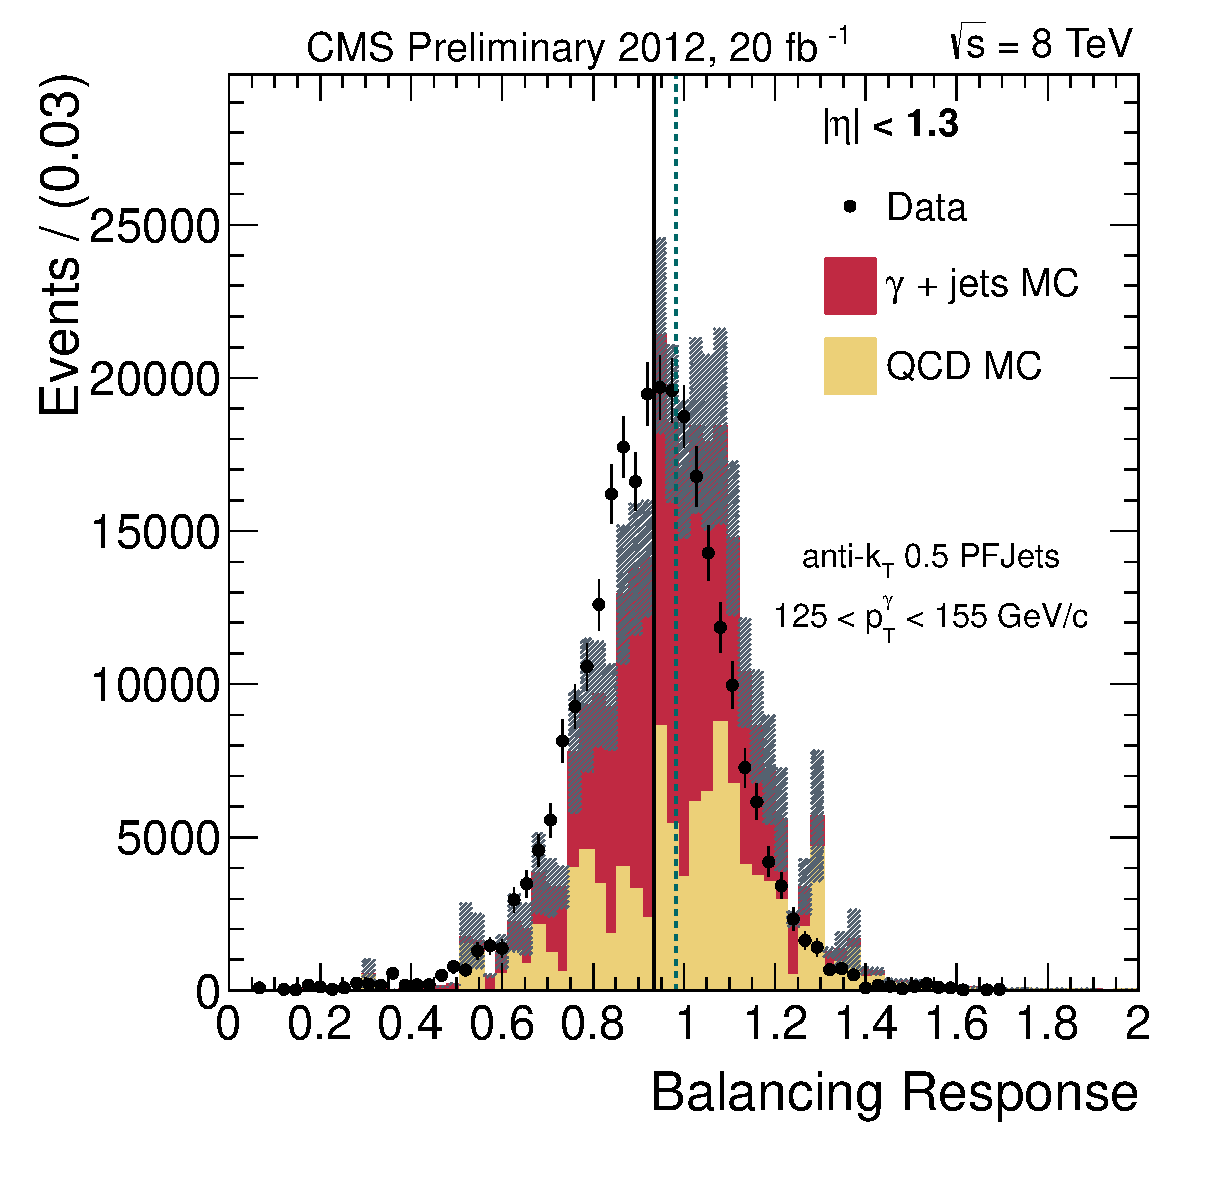
\includegraphics[width=0.45\textwidth]{chapitre4/figs/resp_balancing_eta013_ptPhot_125_155.eps}}\hfill
    \subcaptionbox{\label{fig:bal_eta013_pt_210_250}}[0.45\textwidth]{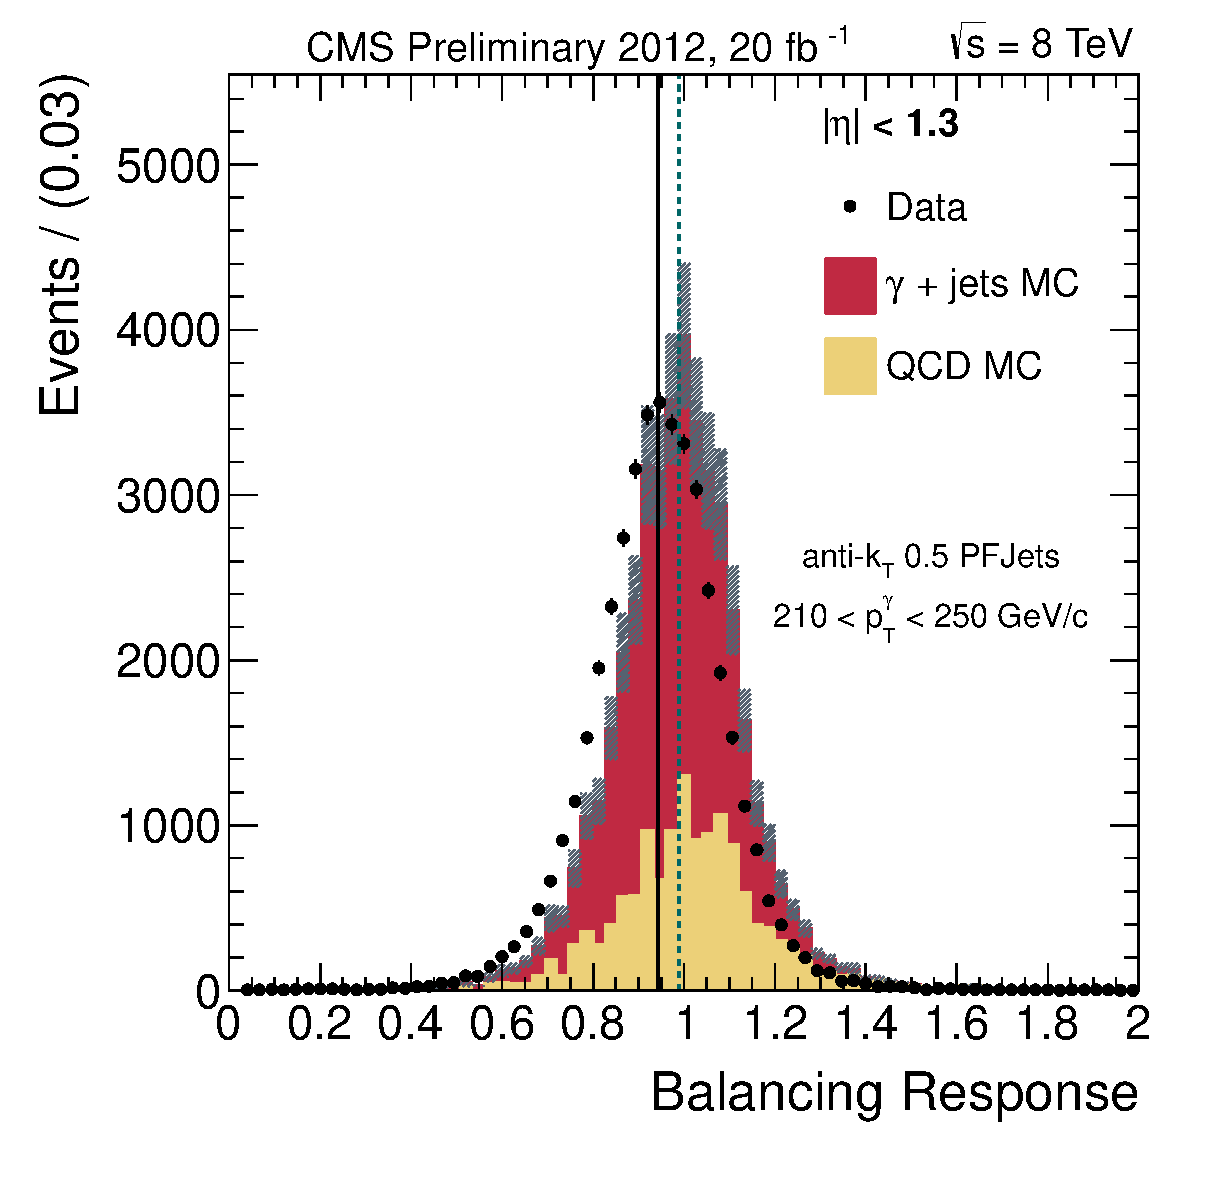
\includegraphics[width=0.45\textwidth]{chapitre4/figs/resp_balancing_eta013_ptPhot_210_250.eps}}
    \subcaptionbox{\label{fig:mpf_eta013_pt_125_155}}[0.45\textwidth]{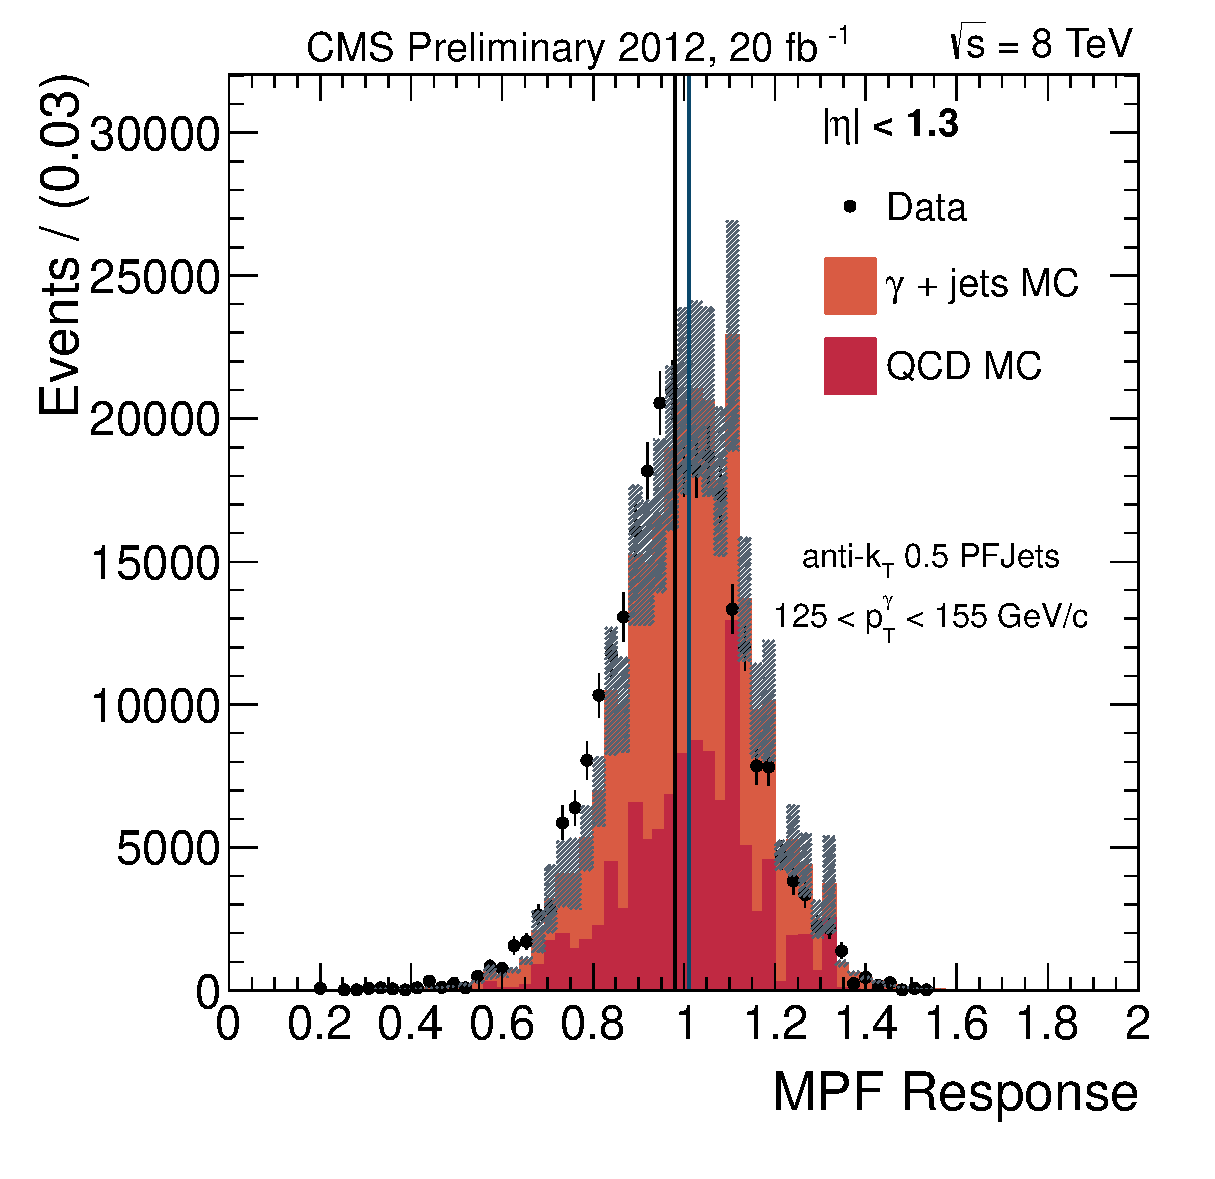
\includegraphics[width=0.45\textwidth]{chapitre4/figs/resp_mpf_eta013_ptPhot_125_155.eps}}\hfill
    \subcaptionbox{\label{fig:mpf_eta013_pt_210_250}}[0.45\textwidth]{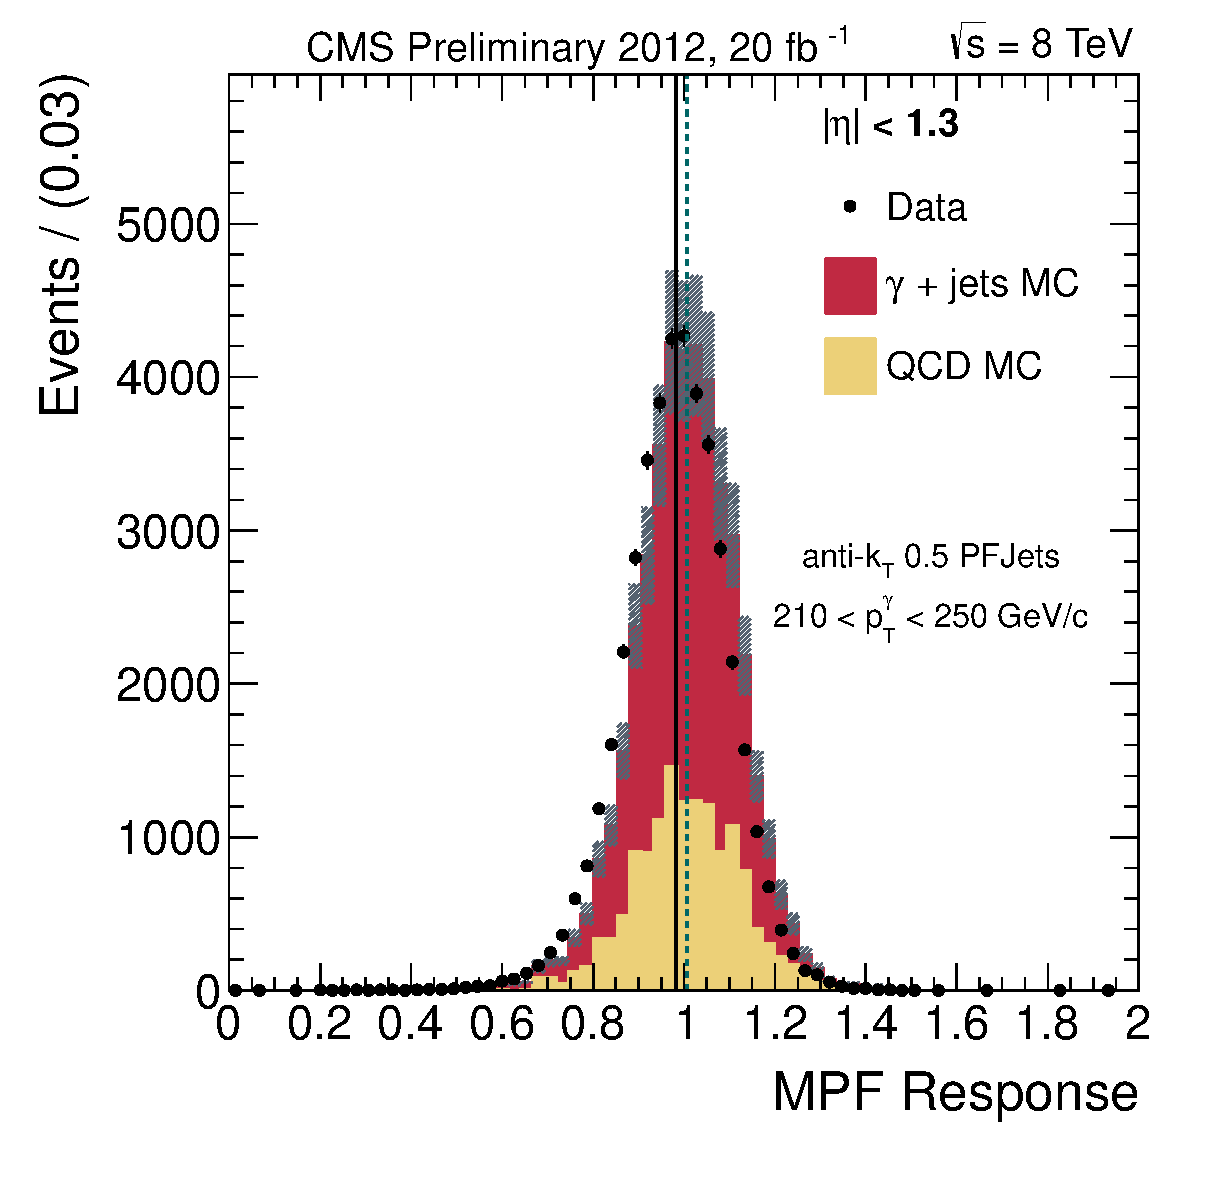
\includegraphics[width=0.45\textwidth]{chapitre4/figs/resp_mpf_eta013_ptPhot_210_250.eps}}
    \caption{Réponses pour la méthode de la balance (haut) et pour la méthode MPF (bas), pour deux classes en \pt : 125 - \SI{155}{\GeV} (gauche) et 210 - \SI{250}{\GeV} (droite). Pour toutes les distributions, $\aeta < \num{1.3}$ Les histogrammes représentent la simulation et les points les données. La ligne noire correspond à la réponse moyenne $R_m$ extraite sur les données et la ligne bleue celle extraite sur la simulation.}
    \label{fig:responses_mpf_balancing}
\end{figure}

\clearpage

\subsection{Résultats}

Pour chaque distribution des réponses, on extrait la réponse moyenne et la résolution. Afin d'extraire les corrections résiduelles, on trace l'évolution de $R_m$ en fonction de l'impulsion transverse du photon, pour les données et la simulation, pour différentes classes en \aeta. En calculant le rapport entre données et simulation, on détermine le facteur de correction à appliquer sur les données.

On définit le facteur de correction $f$ par
\begin{align*}
  f &= \frac{R_m^{\text{simulation}}}{R_m^{\text{données}}}
\end{align*}

En appliquant ce facteur de correction sur les données, on a
\begin{align*}
  f\;R_m^{\text{données}} &= R_m^{\text{simulation}}
\end{align*}
ce qui est effectivement le but recherché.

\bigskip

On présente par la suite les résultats obtenus avec les méthodes de la balance et MPF, avec et sans extrapolation, qui permettent d'extraire le facteur de correction résiduel. Pour chaque méthode, les distributions des réponses moyennes et des résolutions sera présenté pour différentes classes en \aeta.

\subsubsection{Méthode de la balance, sans extrapolation}

On présente \cref{fig:balancing_resp} les distributions des réponses moyennes pour différentes classes en \aeta. Le ratio données sur simulation accompagne ces distributions, ce qui permet d'extraire les facteurs de corrections. Pour ce faire, une interpolation linéaire par une constante est dérivée à l'aide des divers ratio. On trouve aussi \cref{fig:balancing_reso} les distributions des résolutions pour les même classes en \aeta. Même si ces résolutions ne sont pas utilisées pour dériver les corrections résiduelles, elles sont intéressante pour se rendre compte des performances de reconstruction des algorithmes. On s'aperçoit d'ailleurs que les jets sont mieux reconstruit sur la simulation que sur les données. Cet effet donne lieu à une autre série de corrections pour la résolution, qui vise à dégrader la résolution des jets sur la simulation pour correspondre à celle des données.

\begin{figure}[p]
    \centering
    \subcaptionbox{\label{fig:bal_eta008}}[0.45\textwidth]{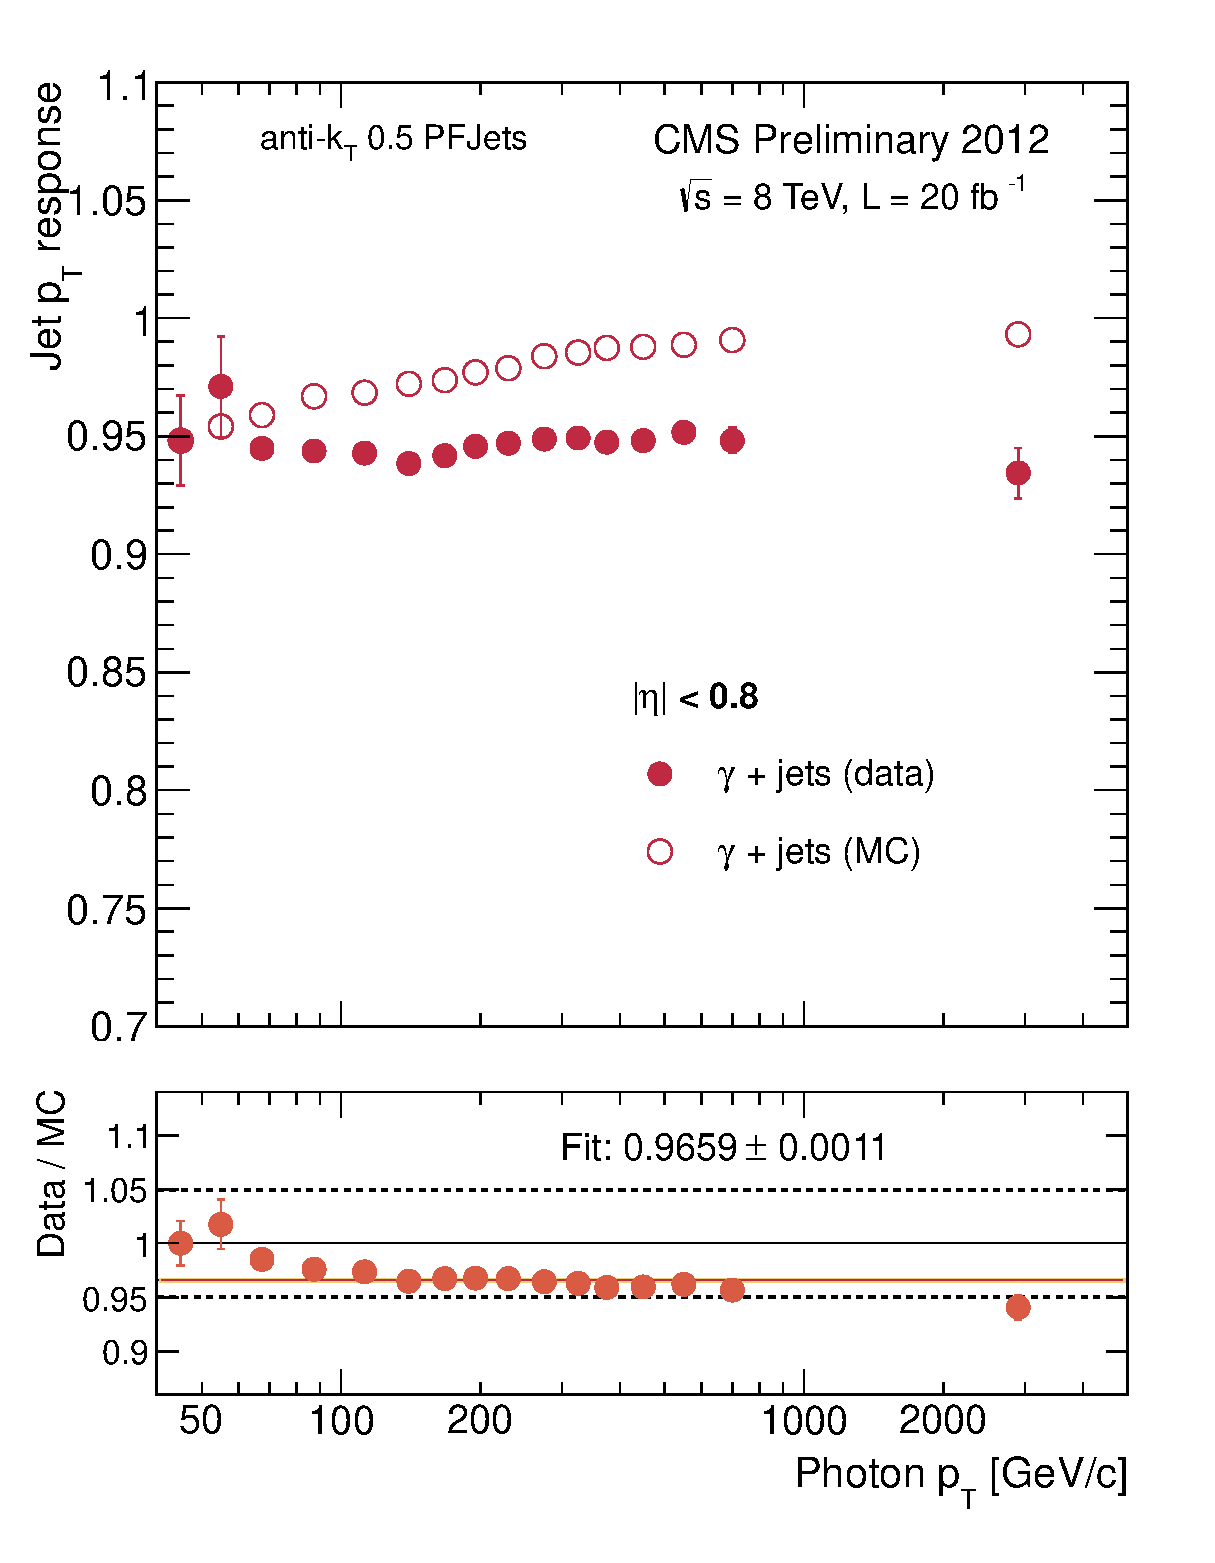
\includegraphics[width=0.45\textwidth]{chapitre4/figs/resp_balancing/response_eta008_balancing.eps}}\hfill
    \subcaptionbox{\label{fig:bal_eta0813}}[0.45\textwidth]{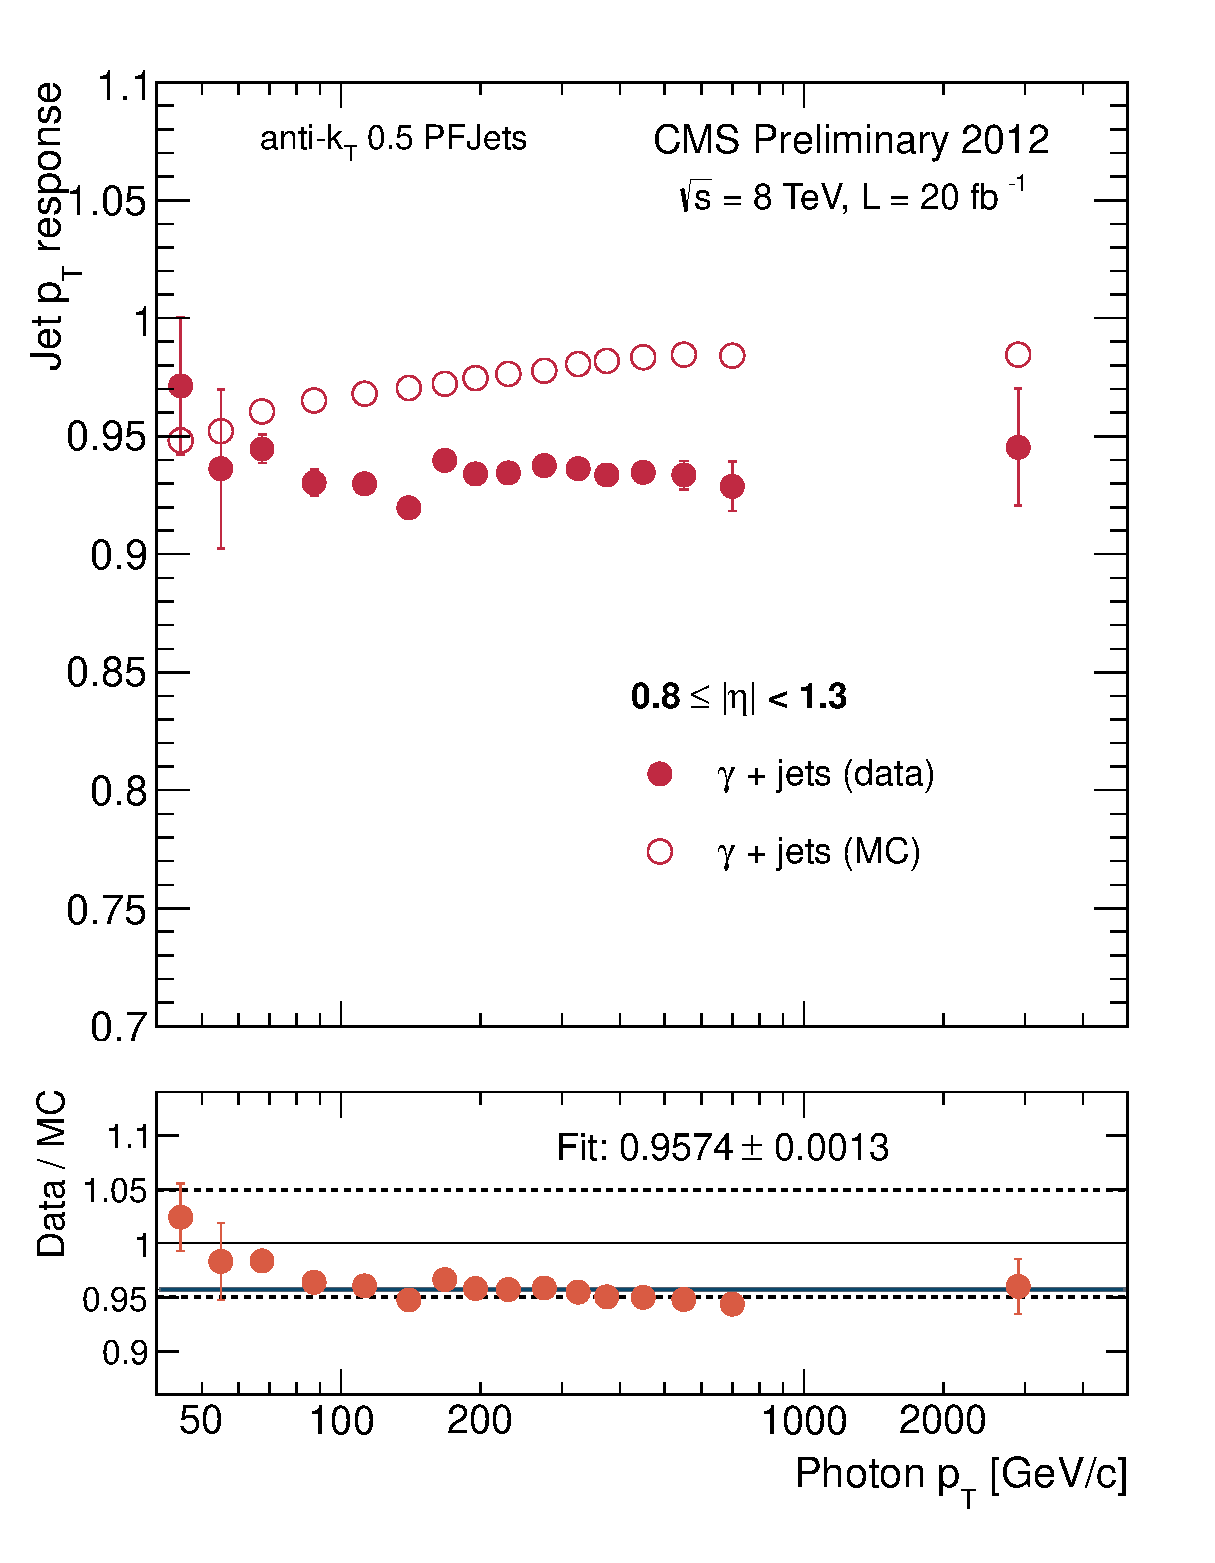
\includegraphics[width=0.45\textwidth]{chapitre4/figs/resp_balancing/response_eta0813_balancing.eps}}
    \subcaptionbox{\label{fig:bal_eta1319}}[0.45\textwidth]{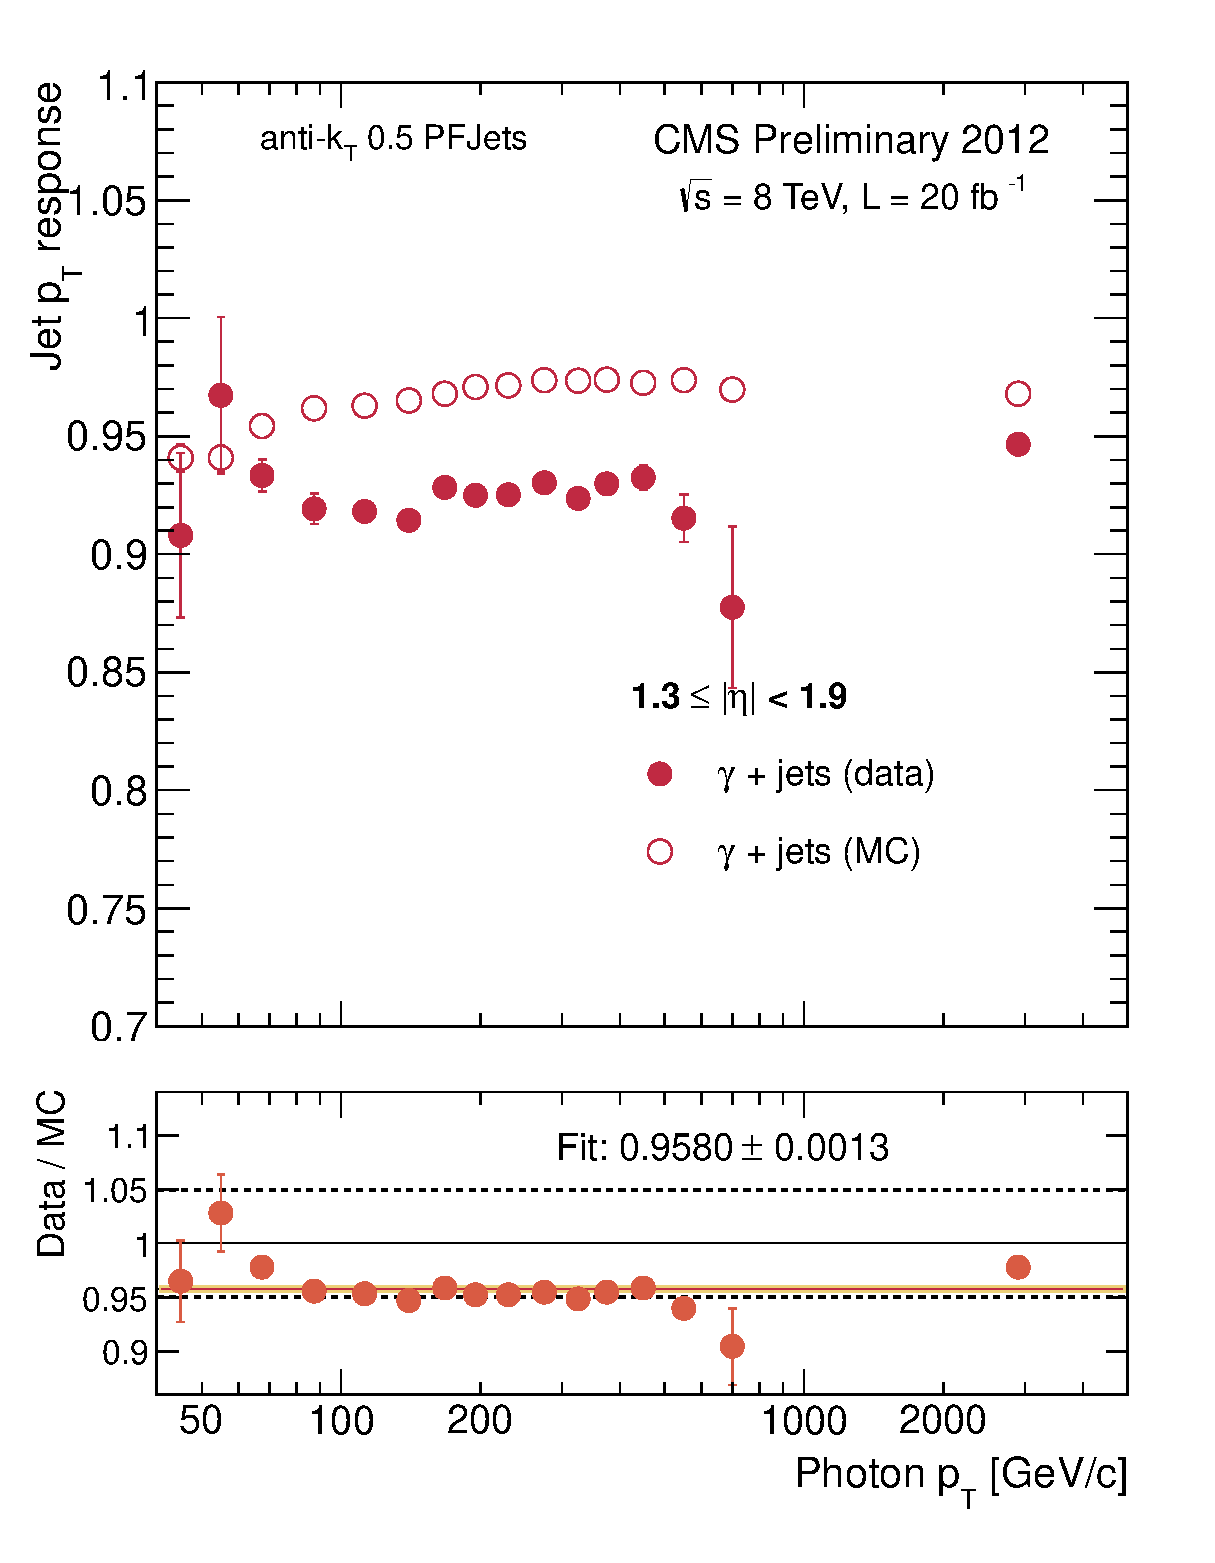
\includegraphics[width=0.45\textwidth]{chapitre4/figs/resp_balancing/response_eta1319_balancing.eps}}\hfill
    \subcaptionbox{\label{fig:bal_eta1925}}[0.45\textwidth]{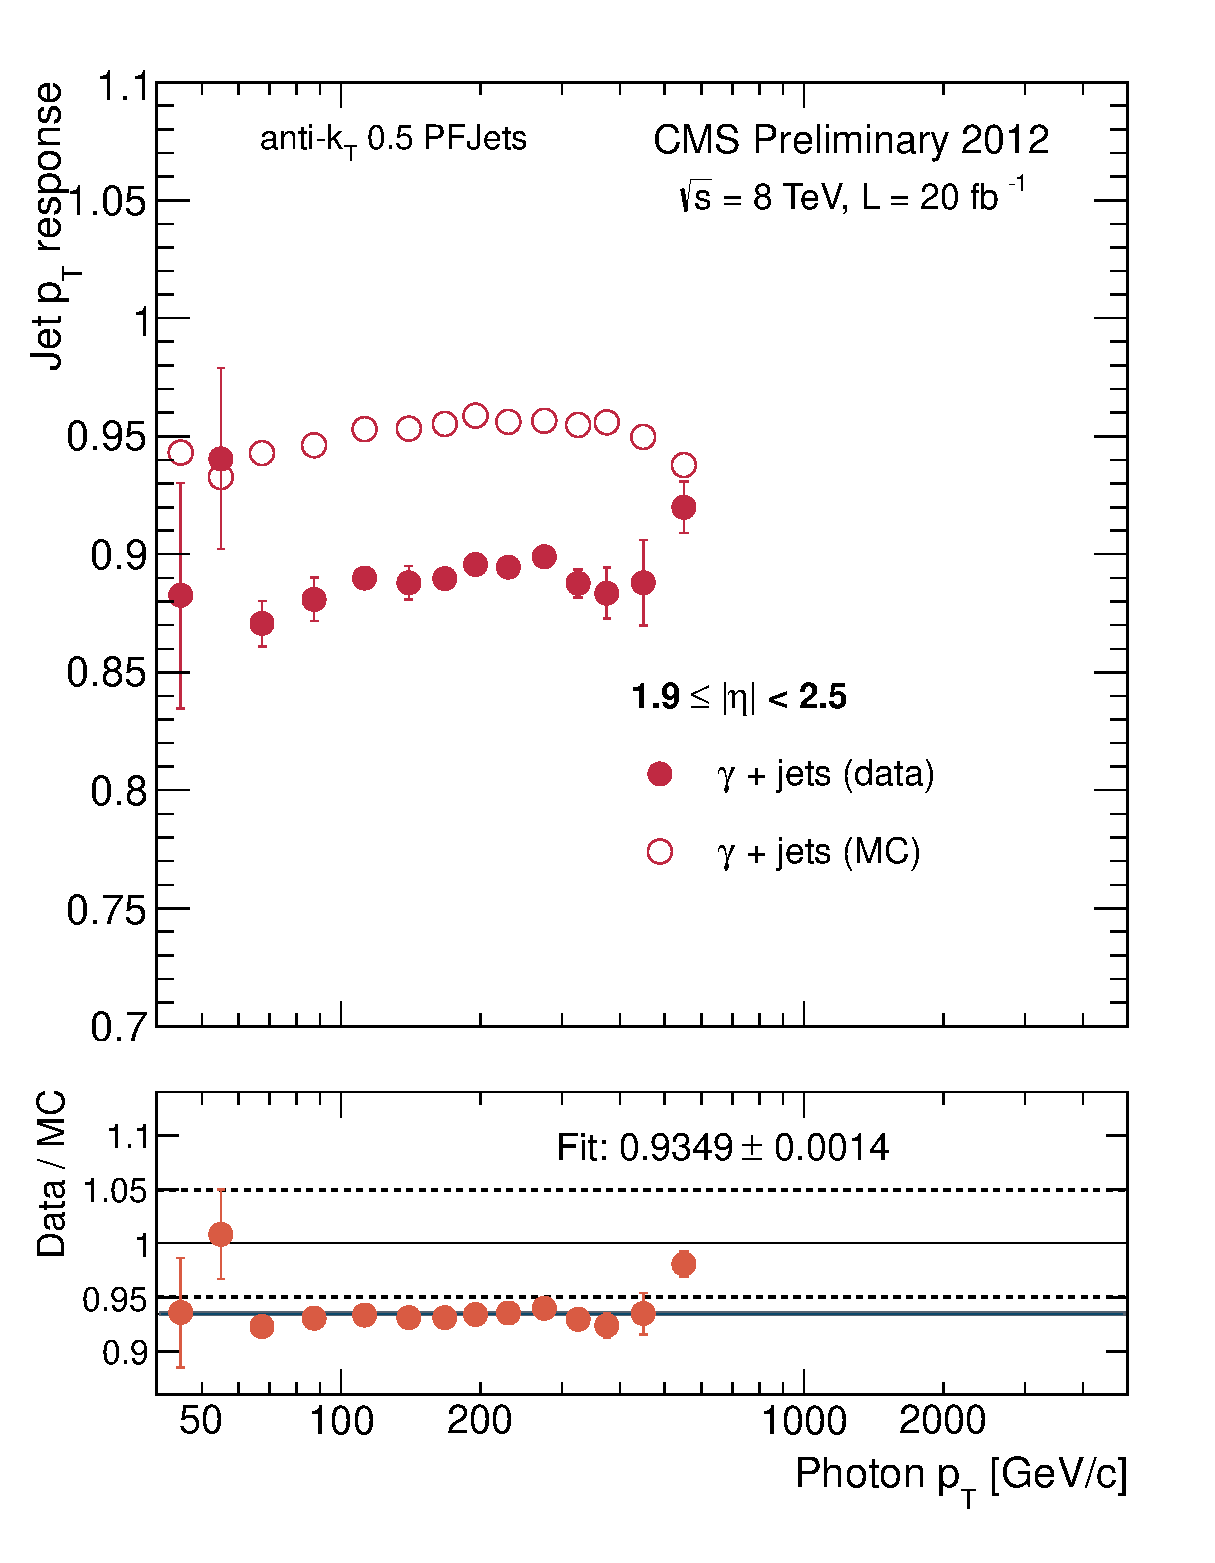
\includegraphics[width=0.45\textwidth]{chapitre4/figs/resp_balancing/response_eta1925_balancing.eps}}
    \caption{Réponses moyennes pour la méthode de la balance pour $\aeta < \num{0.8}$ (\subref{fig:bal_eta008}), $\num{0.8} \leq \aeta < \num{1.3}$ (\subref{fig:bal_eta0813}), $\num{1.3} \leq \aeta < \num{1.9}$ (\subref{fig:bal_eta1319}), et $\num{1.9} \leq \aeta < \num{2.5}$ (\subref{fig:bal_eta1925}). Le ratio entre les données et la simulation est présenté sous chaque distribution, accompagné d'une interpolation linéaire constante (ligne grise)}
    \label{fig:balancing_resp}
\end{figure}

\begin{figure}[p]
    \centering
    \subcaptionbox{\label{fig:reso_bal_eta008}}[0.45\textwidth]{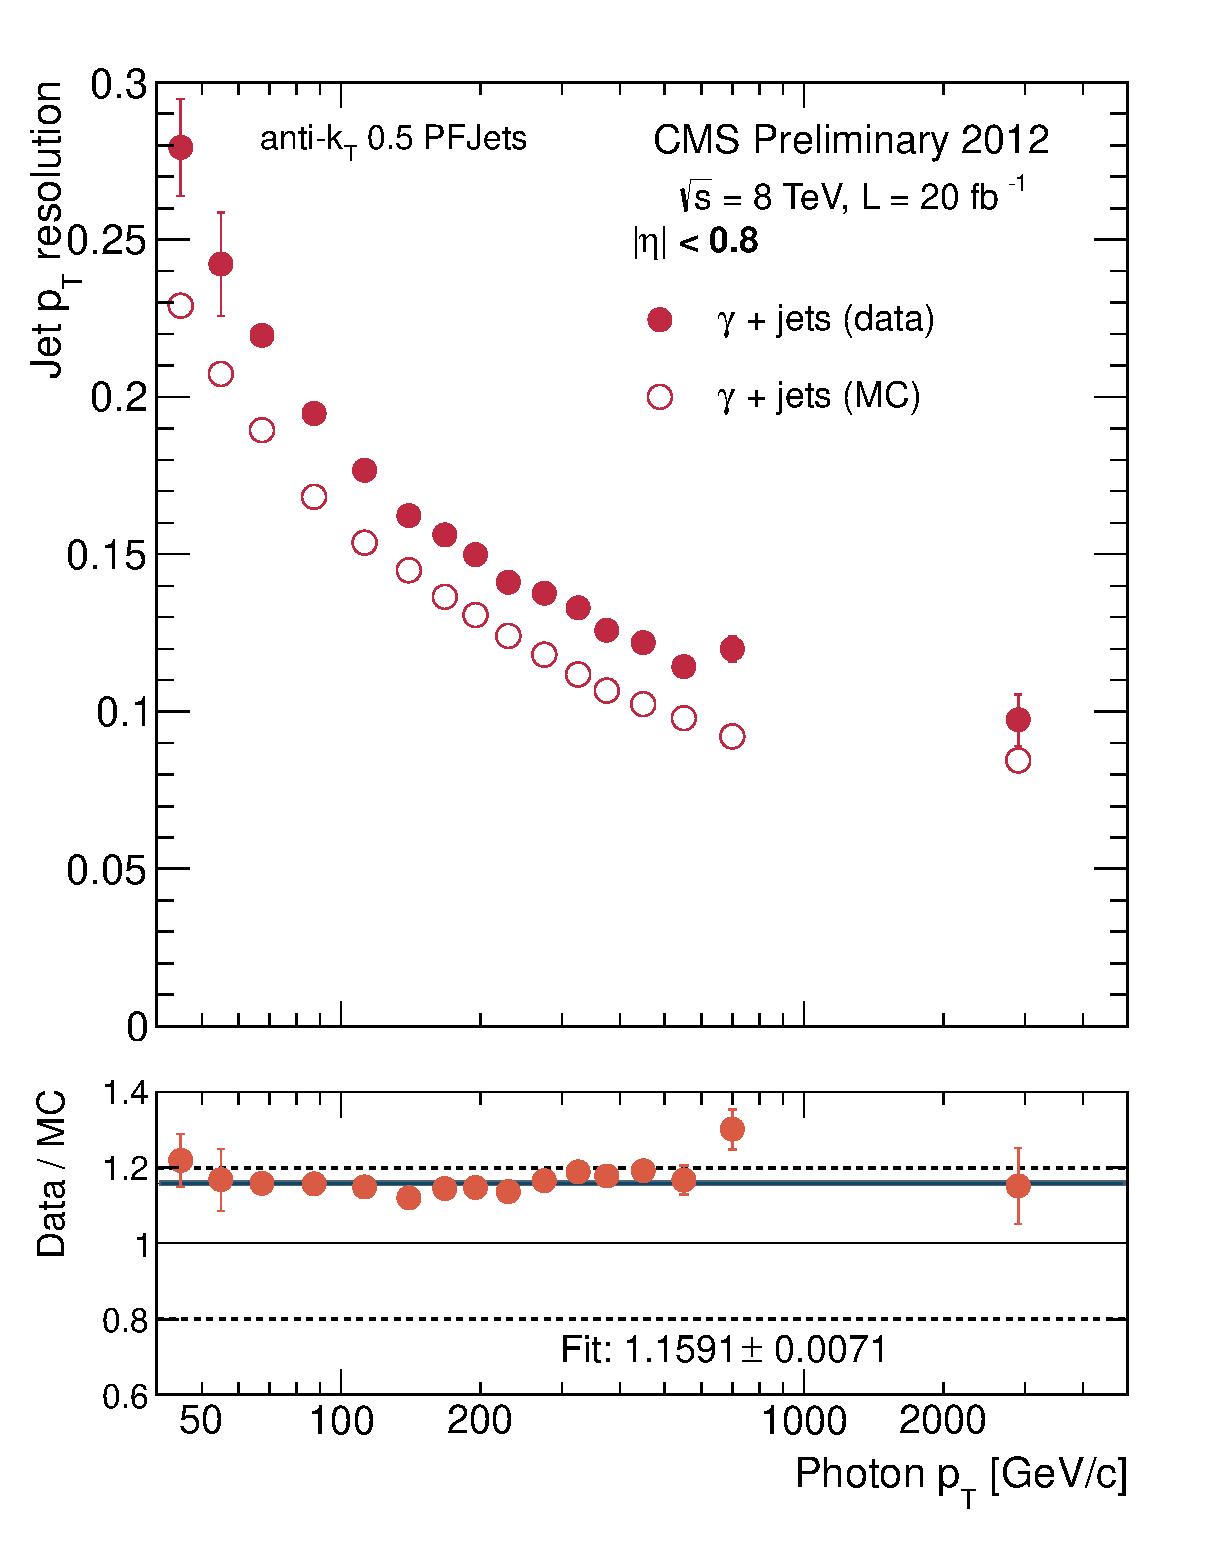
\includegraphics[width=0.45\textwidth]{chapitre4/figs/reso_balancing/resolution_eta008_balancing.eps}}\hfill
    \subcaptionbox{\label{fig:reso_bal_eta0813}}[0.45\textwidth]{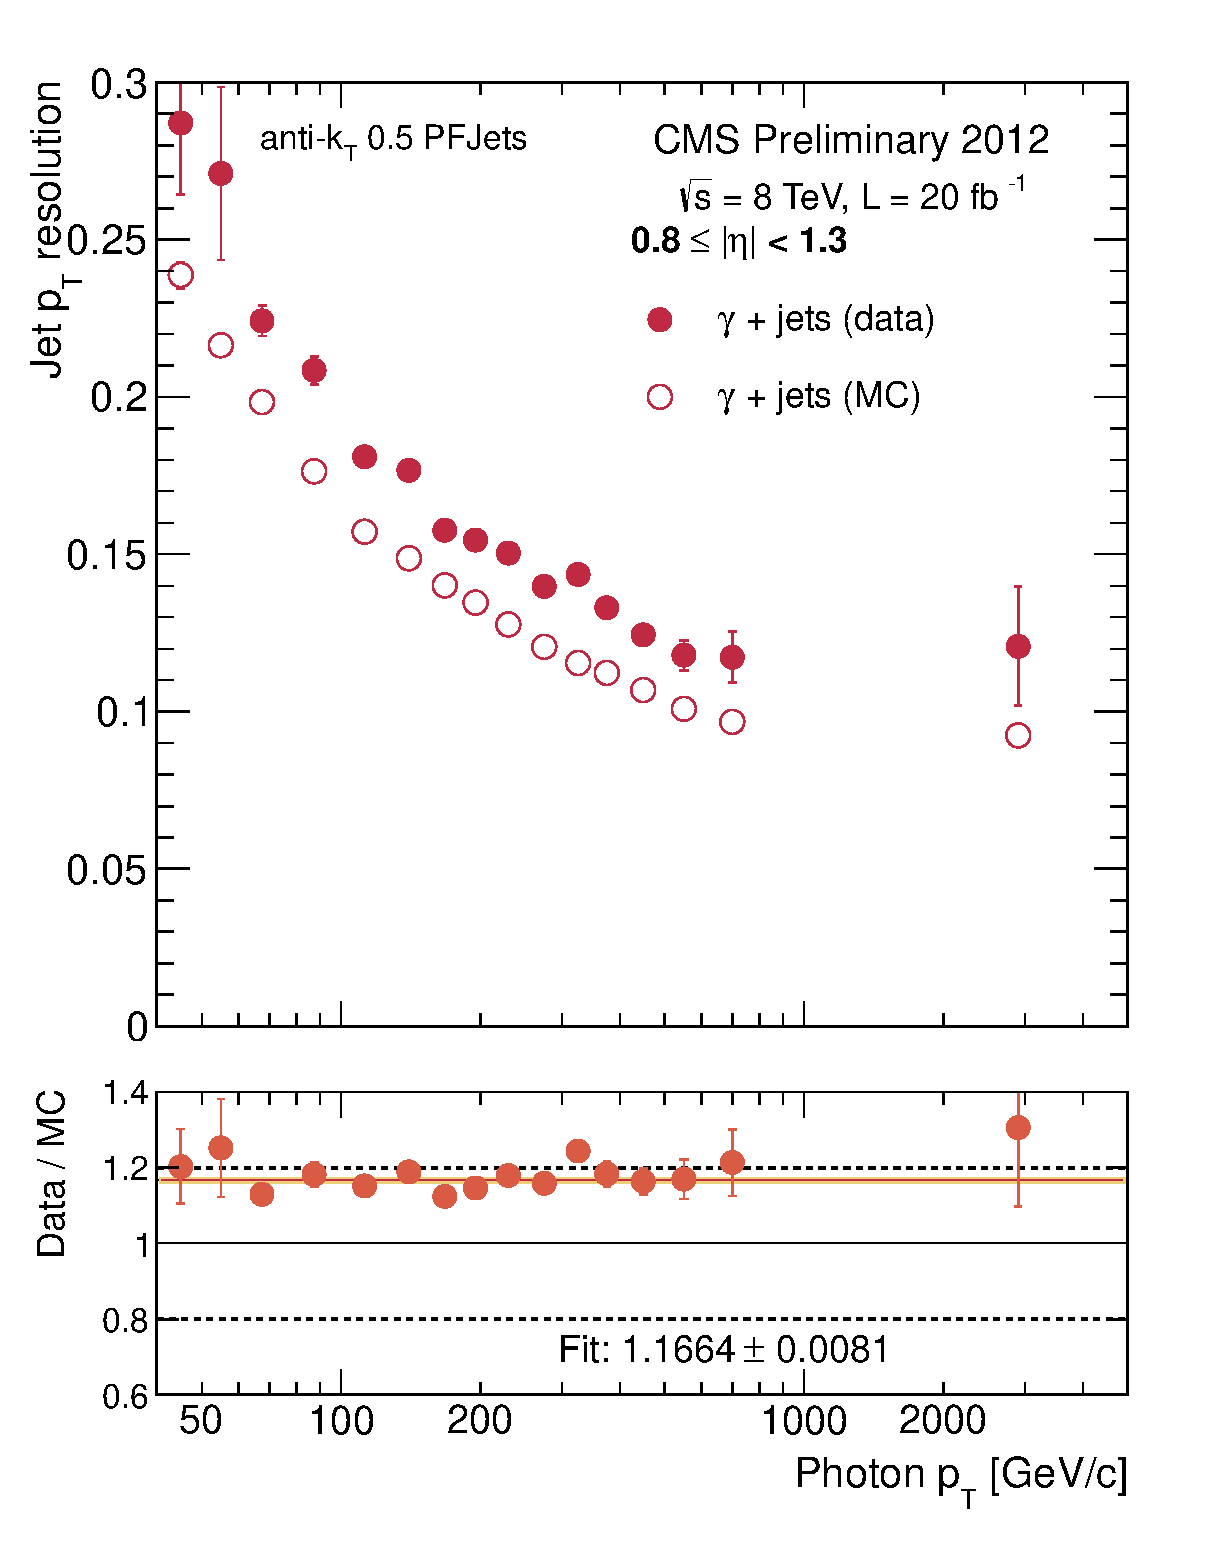
\includegraphics[width=0.45\textwidth]{chapitre4/figs/reso_balancing/resolution_eta0813_balancing.eps}}
    \subcaptionbox{\label{fig:reso_bal_eta1319}}[0.45\textwidth]{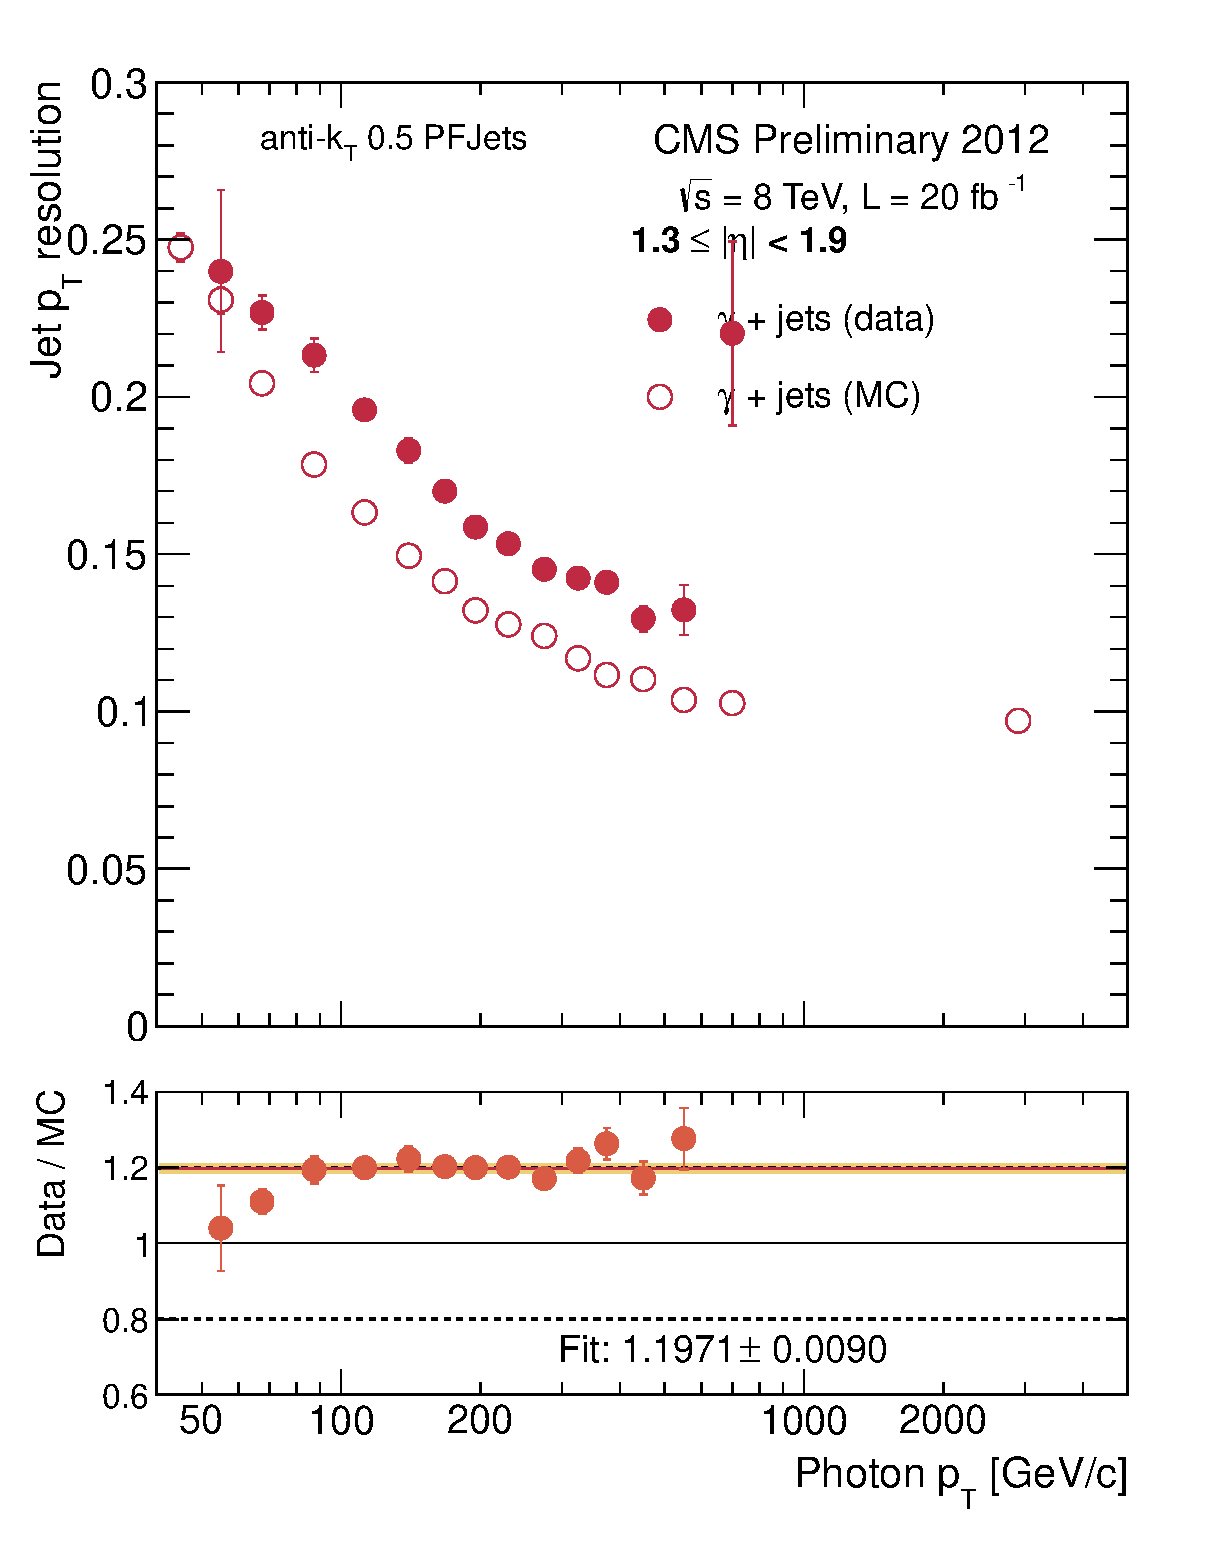
\includegraphics[width=0.45\textwidth]{chapitre4/figs/reso_balancing/resolution_eta1319_balancing.eps}}\hfill
    \subcaptionbox{\label{fig:reso_bal_eta1925}}[0.45\textwidth]{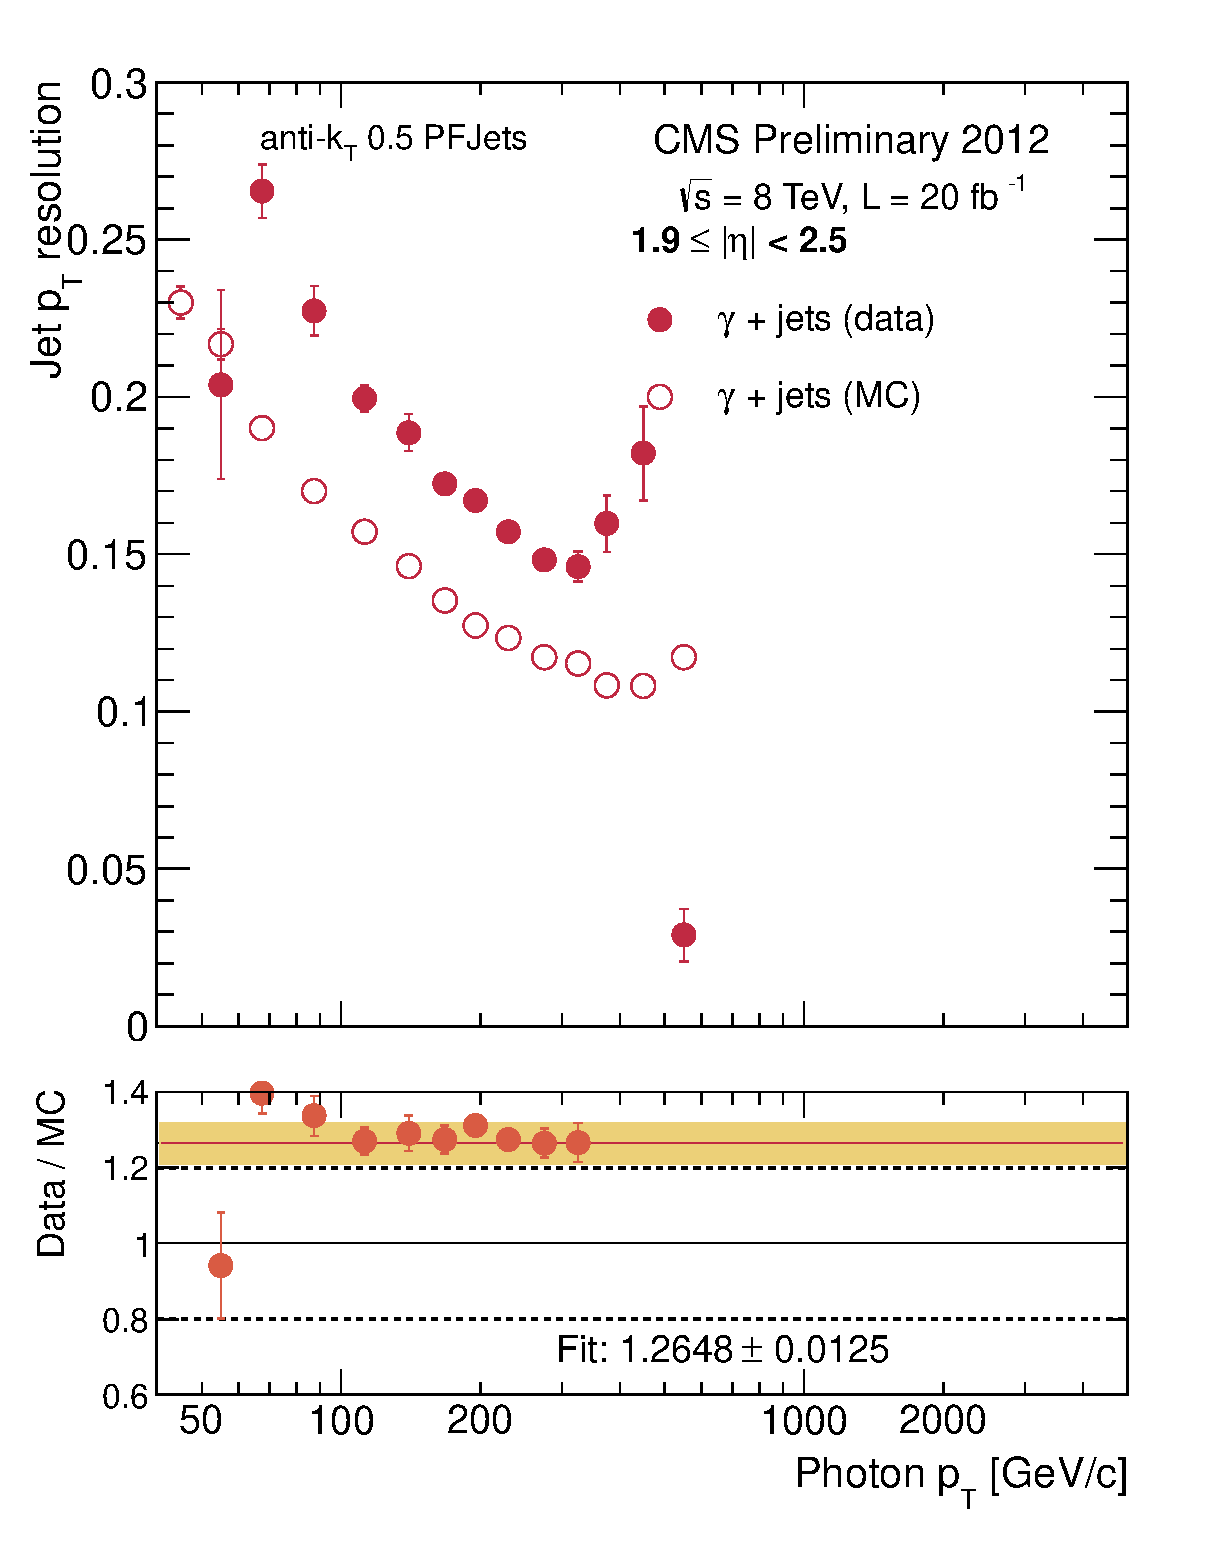
\includegraphics[width=0.45\textwidth]{chapitre4/figs/reso_balancing/resolution_eta1925_balancing.eps}}
    \caption{Résolutions pour la méthode de la balance pour $\aeta < \num{0.8}$ (\subref{fig:reso_bal_eta008}), $\num{0.8} \leq \aeta < \num{1.3}$ (\subref{fig:reso_bal_eta0813}), $\num{1.3} \leq \aeta < \num{1.9}$ (\subref{fig:reso_bal_eta1319}), et $\num{1.9} \leq \aeta < \num{2.5}$ (\subref{fig:reso_bal_eta1925}). Le ratio entre les données et la simulation est présenté sous chaque distribution, accompagné d'une interpolation linéaire constante (ligne grise)}
    \label{fig:balancing_reso}
\end{figure}

\bigskip

On présente dans le \cref{tab:res_balancing} un résumé des ratios et des facteurs de correction extraient pour chaque classe en \aeta.

Le ratio est stable dans le tonneau ($\aeta < \num{2.1}$), avec un facteur de correction d'environ \SI{4}{\%}. Dans les bouchons, le ratio chutent jusqu'à des facteurs de correction atteignant \SI{23}{\%}. Au delà de \SI{3.2}{\radian}, il n'y a plus de trajectographe, et la réponse devient très mauvaise.

\begin{table}[p] \centering
 \begin{tabular}{@{}ccc@{}} \toprule
 Classe en \aeta & ratio & $f$ \\ \midrule
 \num{0} - \num{0.8} & \num{0.9665 \pm 0.0004} & \num{1.0347 \pm 0.0004}\\
 \num{0.8} - \num{1.3} & \num{0.9579 \pm 0.0007} & \num{1.0440 \pm 0.0008}\\
 \num{1.3} - \num{1.9} & \num{0.9590 \pm 0.0007} & \num{1.0428 \pm 0,0008}\\
 \num{1.9} - \num{2.5} & \num{0.9349 \pm 0.0014} & \num{1.0696 \pm 0,0016}\\
 \num{2.5} - \num{3} & \num{0.9099 \pm 0.0035} & \num{1.0990 \pm 0,0042}\\
 \num{3} - \num{3.2} & \num{0.8134 \pm 0.0119} & \num{1.2294 \pm 0,0180}\\
 \num{3.2} - \num{5.2} & \num{0.4286 \pm 0.0005} & \num{2.3331 \pm 0,0027}\\
 \bottomrule
 \end{tabular}
 \caption{Ratios et facteurs de correction pour différentes classes en \aeta obtenus grâce à la méthode de la balance, sans extrapolation.}
 \label{tab:res_balancing}
\end{table}

\begin{table}[p] \centering
 \begin{tabular}{@{}ccc@{}} \toprule
 Classe en \aeta & ratio & $f$ \\ \midrule
 \num{0} - \num{0.8} & \num{0.9665 \pm 0.0004} & \num{1.0347 \pm 0.0004}\\
 \num{0.8} - \num{1.3} & \num{0.9579 \pm 0.0007} & \num{1.0440 \pm 0.0008}\\
 \num{1.3} - \num{1.9} & \num{0.9590 \pm 0.0007} & \num{1.0428 \pm 0,0008}\\
 \num{1.9} - \num{2.5} & \num{0.9349 \pm 0.0014} & \num{1.0696 \pm 0,0016}\\
 \num{2.5} - \num{3} & \num{0.9099 \pm 0.0035} & \num{1.0990 \pm 0,0042}\\
 \num{3} - \num{3.2} & \num{0.8134 \pm 0.0119} & \num{1.2294 \pm 0,0180}\\
 \num{3.2} - \num{5.2} & \num{0.4286 \pm 0.0005} & \num{2.3331 \pm 0,0027}\\
 \bottomrule
 \end{tabular}
 \caption{Ratios et facteurs de correction pour différentes classes en \aeta obtenus grâce à la méthode de la balance, avec extrapolation.}
 \label{tab:res_balancing_extrap}
\end{table}

\clearpage

\subsubsection{Méthode de la balance, avec extrapolation} \label{sec:res_balancing_extrap}

\begin{figure}[tbp]
    \centering
    \subcaptionbox{\label{fig:extrap_balancing}}[0.45\textwidth]{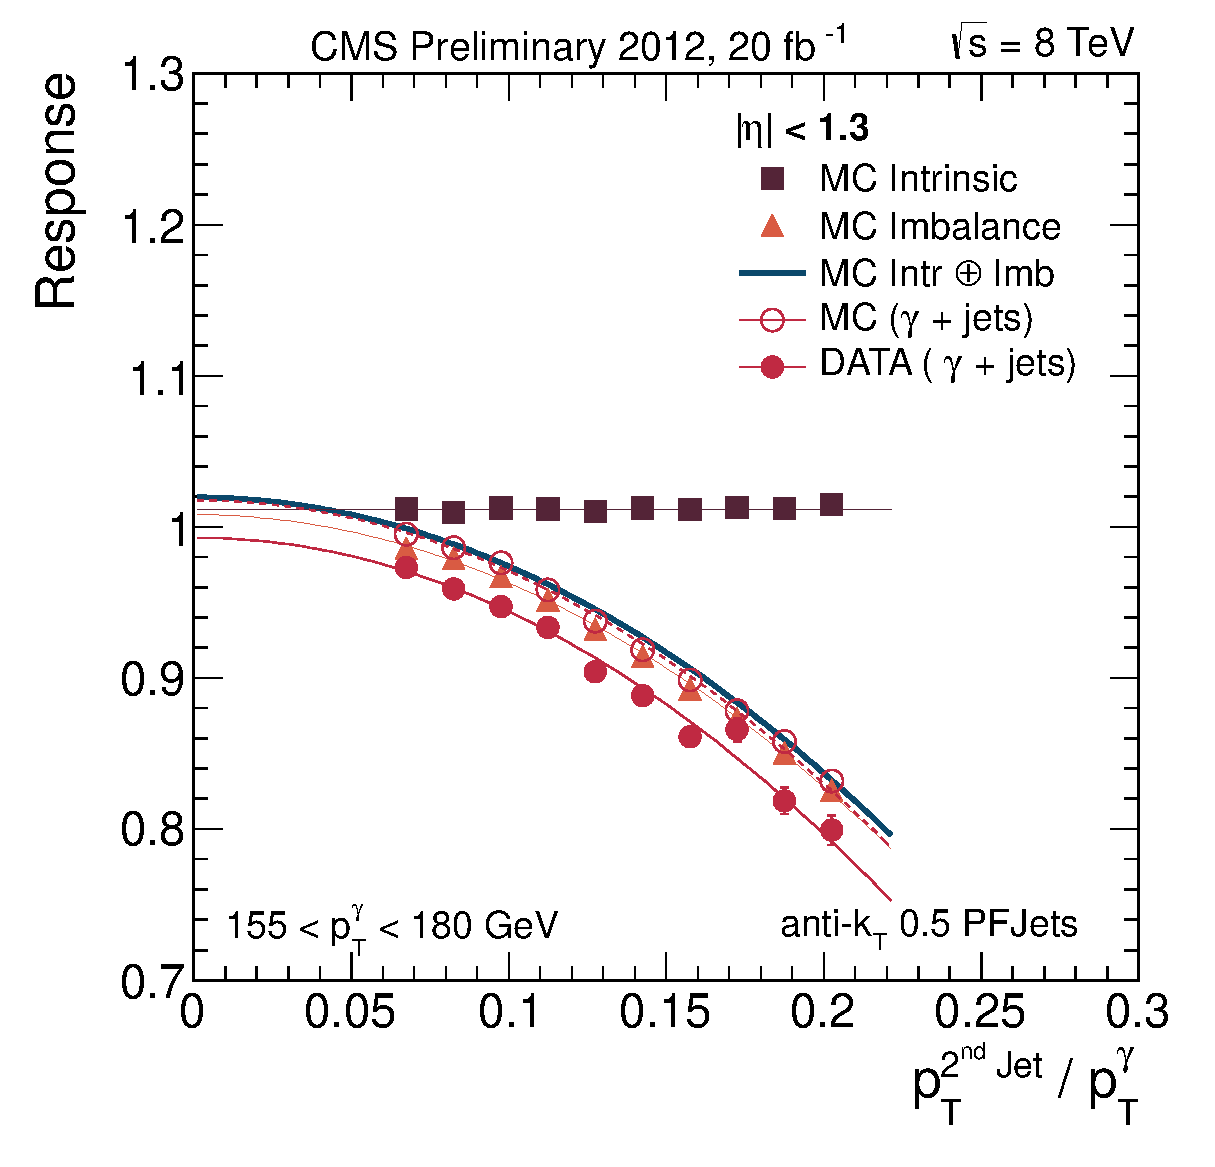
\includegraphics[width=0.45\textwidth]{chapitre4/figs/extrap/response_eta013_ptPhot_155_180.eps}}\hfill
    \subcaptionbox{\label{fig:extrap_mpf}}[0.45\textwidth]{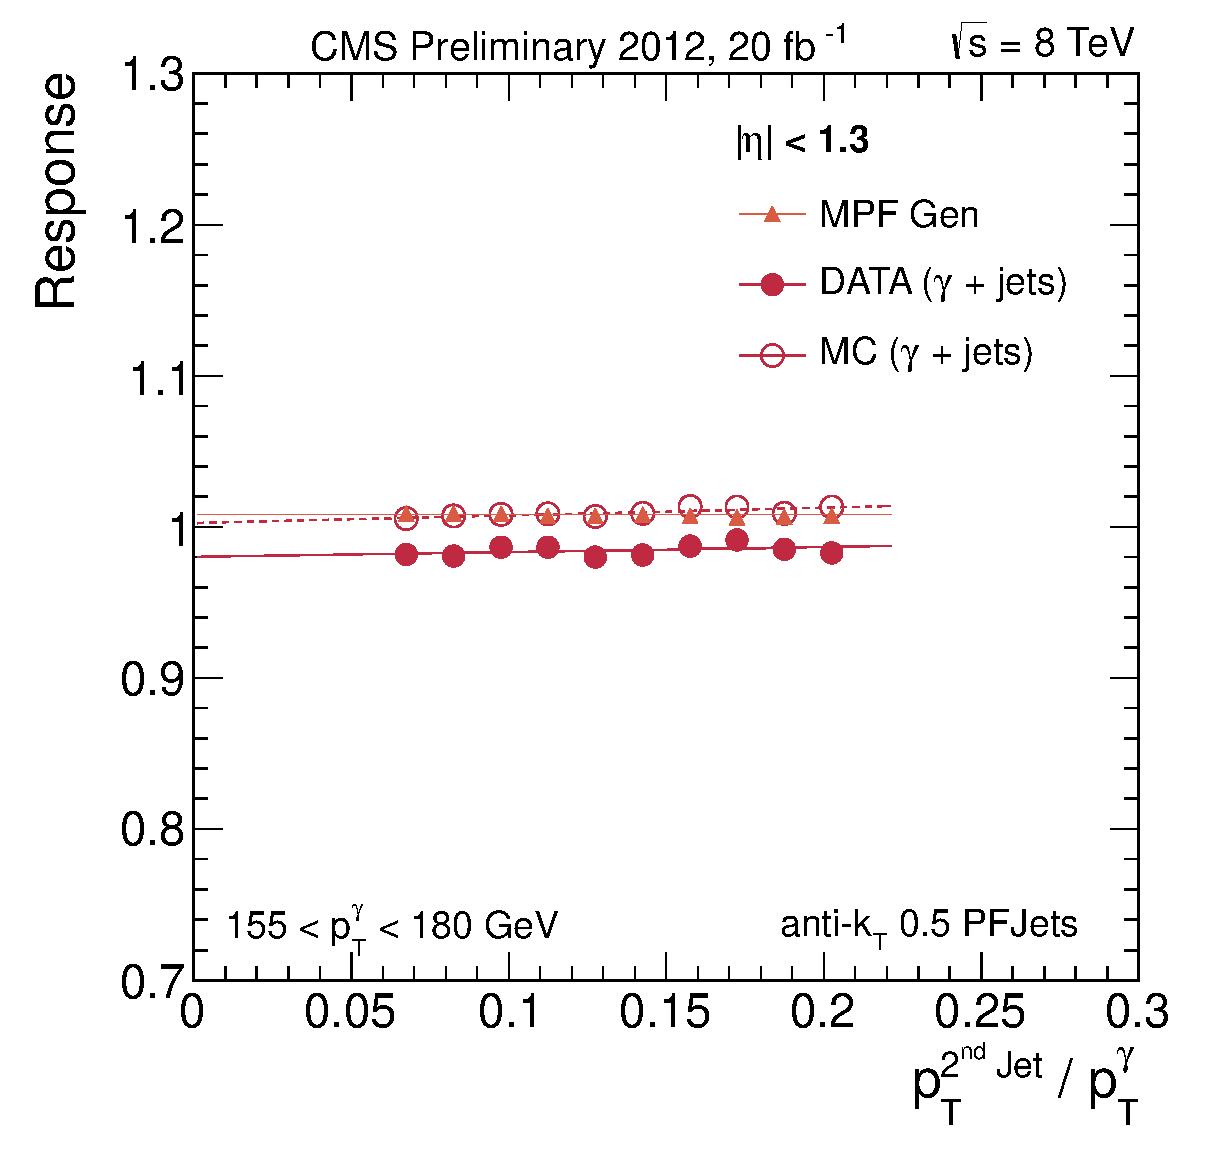
\includegraphics[width=0.45\textwidth]{chapitre4/figs/extrap/responseMPF_eta013_ptPhot_155_180.eps}}
    \caption{Extrapolation de la réponse moyenne pour la méthode de la balance (\subref{fig:extrap_balancing}) et la méthode MPF (\subref{fig:extrap_mpf}). Pour la méthode de la balance, la réponse de la simulation (MC) a été séparée en deux parties, détaillées \cref{sec:res_balancing_extrap}.}
\end{figure}

On a vu précédemment que la méthode de la balance était sensible à la présence de jets additionnels dans l'événement. Afin de contrer cet effet, on extrapole la réponse moyenne à $\alpha \rightarrow 0$. On présente \cref{fig:extrap_balancing} un exemple d'extrapolation pour la méthode de la balance, pour $155 \leq p_T^\gamma < \SI{180}{\GeV}$ et $\aeta < \num{1.3}$, et \cref{fig:extrap_mpf} pour la méthode MPF. On constate une très nette dépendance de la réponse moyenne en fonction de $\alpha$ pour la méthode de la balance, dépendance quasi inexistante pour la méthode MPF.

Pour la méthode de la balance, on sépare la réponse en deux parties. On a
\begin{align*}
  R_m &= \frac{\ptfjet}{\ptg} = \underbrace{ \frac{\ptfjet}{p_T^{\text{\ordinalnum{1} jet généré}}} }_{\text{intrinsèque}} \; \times \; \underbrace{ \frac{p_T^{\text{\ordinalnum{1} jet généré}}}{\ptg} }_{\text{déséquilibre}}
\end{align*}

La partie intrinsèque n'est pas dépendante de la présence de jets additionnels, d'où l'allure plate \cref{fig:extrap_balancing}. Elle est uniquement sensible aux problèmes de calibrations des divers détecteurs, problèmes résolus à l'aide des corrections de niveau 1, 2 et 3. C'est ainsi qu'on obtient une réponse intrinsèque très proche de l'unité.